\documentclass[a4paper]{article}
\usepackage{vntex}
%\usepackage[english,vietnam]{babel}
%\usepackage[utf8]{inputenc}

%\usepackage[utf8]{inputenc}
%\usepackage[francais]{babel}


\usepackage{float}
\usepackage{a4wide,amssymb,epsfig,latexsym,multicol,array,hhline,fancyhdr}
\usepackage{booktabs}
\usepackage{amsmath}
\usepackage{lastpage}
\usepackage[lined,boxed,commentsnumbered]{algorithm2e}
\usepackage{enumerate}
\usepackage{color}
\usepackage{graphicx}							% Standard graphics package
\usepackage{array}
\usepackage{tabularx, caption}
\usepackage{multirow}
\usepackage[framemethod=tikz]{mdframed}% For highlighting paragraph backgrounds
\usepackage{multicol}
\usepackage{rotating}
\usepackage{graphics}
\usepackage{geometry}
\usepackage{setspace}
\usepackage{epsfig}
\usepackage{tikz}
\usepackage{listings}
\usetikzlibrary{arrows,snakes,backgrounds}
\usepackage{hyperref}
\usepackage{scrextend}
\changefontsizes{13pt}
\usepackage{svg}
\usepackage{hyperref}
\usepackage{enumitem}
\usepackage{tocloft}
\renewcommand{\cftsecleader}{\cftdotfill{\cftdotsep}}
\renewcommand{\thesection}{\Roman{section}}
\hypersetup{urlcolor=blue,linkcolor=black,citecolor=black,colorlinks=true} 
%\usepackage{pstcol} 								% PSTricks with the standard color package



\newtheorem{theorem}{{\bf Định lý}}
\newtheorem{property}{{\bf Tính chất}}
\newtheorem{proposition}{{\bf Mệnh đề}}
\newtheorem{corollary}[proposition]{{\bf Hệ quả}}
\newtheorem{lemma}[proposition]{{\bf Bổ đề}}

\everymath{\color{blue}}
%\usepackage{fancyhdr}
\setlength{\headheight}{40pt}
\pagestyle{fancy}
\fancyhead{} % clear all header fields
\fancyhead[L]{
 \begin{tabular}{rl}
    \begin{picture}(25,15)(0,0)
    \put(0,-8){
\includegraphics[width=8mm, height=8mm]{hcmut.png}}
    %\put(0,-8){\epsfig{width=10mm,figure=hcmut.eps}}
   \end{picture}&
	%
\includegraphics[width=8mm, height=8mm]{hcmut.png} & %
	\begin{tabular}{l}
		\textbf{\bf \ttfamily Trường Đại Học Bách Khoa Tp.Hồ Chí Minh}\\
		\textbf{\bf \ttfamily Khoa Khoa Học và Kỹ Thuật Máy Tính}
	\end{tabular} 	
 \end{tabular}
}
\fancyhead[R]{
	\begin{tabular}{l}
		\tiny \bf \\
		\tiny \bf 
	\end{tabular}  }
\fancyfoot{} % clear all footer fields
\fancyfoot[L]{\scriptsize \ttfamily Bài tập lớn môn Mạng máy tính - Niên khóa 2024-2025}
\fancyfoot[R]{\scriptsize \ttfamily Trang {\thepage}/\pageref{LastPage}}
\renewcommand{\headrulewidth}{0.3pt}
\renewcommand{\footrulewidth}{0.3pt}


%%%
\setcounter{secnumdepth}{4}
\setcounter{tocdepth}{3}
\makeatletter
\newcounter {subsubsubsection}[subsubsection]
\renewcommand\thesubsubsubsection{\thesubsubsection .\@alph\c@subsubsubsection}
\newcommand\subsubsubsection{\@startsection{subsubsubsection}{4}{\z@}%
                                     {-3.25ex\@plus -1ex \@minus -.2ex}%
                                     {1.5ex \@plus .2ex}%
                                     {\normalfont\normalsize\bfseries}}
\newcommand*\l@subsubsubsection{\@dottedtocline{3}{10.0em}{4.1em}}
\newcommand*{\subsubsubsectionmark}[1]{}
\makeatother

\definecolor{dkgreen}{rgb}{0,0.6,0}
\definecolor{gray}{rgb}{0.5,0.5,0.5}
\definecolor{mauve}{rgb}{0.58,0,0.82}
\definecolor{backcolor}{RGB}{212,235,242}
\lstset{frame=tb,
	language=R,
	aboveskip=3mm,
	belowskip=3mm,
	showstringspaces=false,
	columns=flexible,
	basicstyle={\small\ttfamily},
	numbers=none,
	numberstyle=\tiny\color{gray},
	keywordstyle=\color{blue},
	commentstyle=\color{dkgreen},
	stringstyle=\color{mauve},
	breaklines=true,
	breakatwhitespace=true,
	tabsize=3,
	numbers=left,
	stepnumber=1,
	numbersep=1pt,    
	firstnumber=1,
	numberfirstline=true,
}

\usepackage{indentfirst}

% \documentclass{article}

\everymath{\color{black}} % Đặt màu đen cho chế độ toán học
\everydisplay{\color{black}} % Đặt màu đen cho môi trường toán học hiển thị

\renewcommand{\thesection}{\arabic{section}}

\begin{document}
\setlength{\parindent}{0.5cm}

\begin{titlepage}
\begin{center}
ĐẠI HỌC QUỐC GIA THÀNH PHỐ HỒ CHÍ MINH \\
TRƯỜNG ĐẠI HỌC BÁCH KHOA \\
KHOA KHOA HỌC - KỸ THUẬT MÁY TÍNH 
\end{center}

\begin{figure}[h!]
\begin{center}

\includegraphics[scale = 0.27]{01_logobachkhoasang.png}
\end{center}
\end{figure}


\begin{center}
\begin{tabular}{c}
	\multicolumn{1}{l}{\textbf{{\Large HỌC KỲ 241}}}\\
	~~\\
	\hline
	\\
	\multicolumn{1}{l}{\textbf{{\Large Bài tập lớn}}}\\
	\\
	
	\textbf{{\Huge Computer Network}}\\
	\\
	\hline
\end{tabular}
\end{center}

\begin{table}[h]
\begin{tabular}{rrll}
\hspace{2.5 cm} & GVHD: &  Hoàng Lê Hải Thanh\\
& SV: &  &\\
& &   Huỳnh Minh Khoa&- 2252346\\
& &Thân Nguyễn Minh Khoa &- 2252361\\
& & Trần Lương Yến Nhi &- 2252586\\
 & & Nguyễn Lê Vân Tú&- 2252881\\
\end{tabular}
\end{table}

\begin{center}
{\footnotesize TP. HỒ CHÍ MINH, THÁNG 11/2024}
\end{center}
\end{titlepage}

\newpage
\tableofcontents
\newpage

\section{Chức năng của ứng dụng}
\subsection{Các chức năng ứng dụng để chia sẻ tệp BitTorrent}
    \textbf{File Discovery và chia sẻ Metadata}  
    \textit{Mô tả:} Cho phép người dùng định vị và truy xuất dữ liệu về thông tin của các tệp được chia sẻ hoặc tải xuống, thường thông qua các tệp .torrent hoặc magnet link.  

    \textbf{Peer Discovery}  
    \textit{Mô tả:} Cho phép nhận dạng và kết nối với các peer khác đang chia sẻ cùng một tệp, đảm bảo chia sẻ phân tán.  


    \textbf{Phân phối tập tin}  
    \textit{Mô tả:} Chia tệp thành các mảnh nhỏ hơn để chia sẻ hiệu quả. Mỗi mảnh được chia sẻ và xác minh riêng lẻ để đảm bảo tính toàn vẹn của dữ liệu.  
    

    \textbf{Tải lên}  
    \textit{Mô tả:} Xử lý việc gửi các phần tệp từ thiết bị của người dùng đến nhiều peer trong mạng. Đảm bảo cân bằng sự đóng góp và chia sẻ tài nguyên.  
    

    \textbf{Tải xuống}  
    \textit{Mô tả:} Quản lý việc nhận các mảnh tệp từ các peer khác. Đảm bảo sử dụng tối ưu tài nguyên mạng bằng cách tải xuống từ nhiều peer đồng thời.  
    

    \textbf{Xác minh mảnh}  
    \textit{Mô tả:} Xác minh tính toàn vẹn của từng mảnh được tải xuống bằng cách so sánh giá trị băm của nó với giá trị mong đợi, đảm bảo độ tin cậy của quá trình tải xuống.  
    

    \textbf{Xử lý lỗi và phục hồi}  
    \textit{Mô tả:} Phát hiện và phục hồi các sự cố như tải xuống không đầy đủ hoặc bị hỏng. Thử lại các lần tải xuống không thành công và yêu cầu lại các phần bị thiếu từ các peer khác.  
    
\subsection{Chức năng dành riêng cho Tracker}

    \textbf{Đăng kí Peer mới với Tracker}  
    \textit{Mô tả:} Đăng ký peer mới vào mạng chia sẻ tệp để truy xuất thông tin khi cần thi. 
    

    \textbf{Thông báo Tracker}  
    \textit{Mô tả:} Cập nhật trình theo dõi với trạng thái của peer, chẳng hạn như tiến trình tải lên/tải xuống, các tệp mà máy Client đang seeding và trạng thái kết nối.  
    
    \textbf{Truy xuất danh sách các Peer có file từ Tracker}  
    \textit{Mô tả:} Cho phép các peer lấy danh sách các peer khác chia sẻ cùng một tệp từ Tracker.  
    

\section{Giao thức}

    \subsection{Giao thức giữa các Client với nhiệm vụ là Uploader - Downloader}
        \subsubsection{Giao thức tải file khi dùng socket} 
        Lần lượt chờ đợi tin nhắn của nhau ứng theo các trường cần lưu
        \newline
        \newline
            \textbf{B1}: Downloader kết nối với Uploader:
                \begin{itemize}
                    \item Downloader: Client gửi kết nối
                    \item Uploader: Gửi lại message: \textquotedblleft\textquotedblleft Got connection from\textquotedblright{} $+$ client\_addr\textquotedblright{} để xác nhận.
                \end{itemize}
            \textbf{B2}: Downloader sau khi nhận tin xác nhận kết nối sẽ bắt đầu tải file từ Uploader:
                \begin{itemize}
                    \item Downloader: Gửi message: reponame (với reponame là torrent hash)
                    \item Uploader: Từ reponame truy suất ra một mảng mà các phần tử là giá trị nhị phân tượng trưng cho các Piece mà Uploader đã tải xuống
                \end{itemize}
            \textbf{B3}: Downloader chọn chunk muốn được tải từ Uploader:
                Uploader sẽ nằm trong vòng lặp chờ nhận các integer cho đến khi ngắt kết nối:
                \begin{itemize}
                    \item B3.1: Downloader: Sẽ gửi 1 interger ứng với vị trí Piece cần tải
                    \item B3.2: Uploader: Sau khi nhận sẽ bắt đầu gửi dữ liệu từ file theo các Piece với độ dài theo Piece\_length được lưu trong file Torrent cho Downloader
                    \item B3.3: Downloader: Sẽ nhận và xử lý dữ liệu và lập lại bước 3.1 cho đến khi hết Piece để download từ Uploader này hoặc đã tải hết tất cả các Piece
                \end{itemize}
        \subsubsection{Lý do sử dụng socket}
        \begin{itemize}
            \item Socket cho phép kết nối trực tiếp giữa các thiết bị, giúp truyền dữ liệu nhanh chóng và hiệu quả.
            \item Socket cung cấp tốc độ và hiệu quả cao nhờ giao thức TCP đảm bảo độ tin cậy và đúng thứ tự, cũng như có thể kiểm soát chặt chẽ việc truyền tải và linh hoạt chọn giữa các giao thức như TCP hoặc UDP tùy theo nhu cầu.
            \item Socket cho phép truyền tải dữ liệu hai chiều, tức là cả hai bên (client và server) đều có thể gửi và nhận dữ liệu qua đó thuận tiện cho việc trao đổi liên tục giữa Uploader và Downloader.
            \item Sockets cho phép các ứng dụng có thể thực hiện nhiều kết nối đồng thời (thông qua các thư viện hỗ trợ như threading, asyncio trong Python), giúp tăng cường khả năng xử lý của ứng dụng. Ví dụ: một máy chủ có thể sử dụng socket để xử lý nhiều yêu cầu từ nhiều client cùng lúc mà không bị gián đoạn.
            \item Socket có thể được sử dụng trên nhiều hệ điều hành và nền tảng khác nhau như Windows, macOS, Linux, và các thiết bị di động. Điều này giúp ứng dụng mạng sử dụng socket có thể dễ dàng tương thích và hoạt động trên nhiều thiết bị khác nhau.
        \end{itemize}

    \subsection{Giao thức Client - Tracker}
    Được xây dụng dựa trên giao thức HTTP, các client gửi các thông báo đến tracker thông qua giao thức HTTP GET \textquotedblleft \/announce\textquotedblright $+$ /<command> \textquotedblright $+$ \textquotedblleft $?$ \textquotedblright $+$  tham số
    \subsubsection{Các giao thức để Client thông báo Tracker}
    \begin{itemize}
        \item Client tham gia vào Tracker:
        \begin{itemize}
            \item \textquotedblleft/announce/join$?$peerid=BKU$-$Torrent$-$836763067317\&port$=$8333\textquotedblright
            \item Tracker sẽ dựa vào peerid để đưa Client vào swarm và lưu lại port mà client đang mở để chấp nhận kết nối từ các client khác.
        \end{itemize}
        \item Client thông báo có đủ file cho Tracker:
        \begin{itemize}
            \item \textquotedblleft/announce/have?torrent\_hash$=$\%C1\%27\%12\%94\%D7\%F6\%CB5\%94\%FB\%09 \%10\%7Bs\%C1\%BF\%85\%24\%16B\&peerid$=$BKU$-$Torrent$-$836763067317\textquotedblright
            \item Tracker sẽ lưu thông tin của client có peerid đang chia sẻ file theo tham số torrent\_hash là mã hash đại diện cho file torrent đó.
        \end{itemize}
        \item Client thông báo muốn tải file cho Tracker:
        \begin{itemize}
            \item \textquotedblleft/announce/down?torrent\_hash\=\%C1\%27\%12\%94\%D7\%F6\%CB5\%94\%FB\%09 \%10\%7Bs\%C1\%BF\%85\%24\%16B\&peerid$=$BKU$-$Torrent$-$836763067317\textquotedblright
            \item Tracker sẽ dựa vào torrent\_hash để gửi cho peerid một danh sách các IP và port của các client đang có file và đồng thời thêm peerid vào danh sách đó.
        \end{itemize}
        \item Client thông báo thoát khỏi Tracker:
        \begin{itemize}
            \item \textquotedblleft/announce/exit?peerid\=BKU\-Torrent\-836763067317\textquotedblright
            \item Tracker sẽ xóa peerid ra khỏi swarm và danh sách các file mà peerid có.
        \end{itemize}
        \item Client kiểm tra Tracker có hoạt động:
        \begin{itemize}
            \item \textquotedblleft/announce/ping\textquotedblright
            \item Tracker sẽ trả về \textquotedblleft OK\textquotedblright nếu còn hoạt động.
        \end{itemize}
    \end{itemize}
\subsubsection{Một số lý do chính khi dùng HTTP để giao tiếp giữa client và tracker trong BitTorrent:}
\textbf{Phổ biến và dễ triển khai}
\begin{itemize}
    \item HTTP là giao thức phổ biến và đã được sử dụng rộng rãi, hỗ trợ trên hầu hết các mạng và thiết bị. Điều này giúp việc triển khai tracker dễ dàng hơn vì có thể sử dụng cơ sở hạ tầng mạng sẵn có, như các máy chủ web và cổng HTTP.
\end{itemize}

\textbf{Tương thích tốt với tường lửa và NAT}
\begin{itemize}
    \item HTTP hoạt động trên cổng 80 hoặc 443, các cổng này thường được mở trên hầu hết các tường lửa và thiết bị NAT. Điều này giúp client dễ dàng kết nối với tracker mà ít gặp trở ngại, tránh được các hạn chế mạng mà các giao thức không phổ biến hơn có thể gặp phải.
\end{itemize}

\textbf{Dễ mở rộng và hỗ trợ}
\begin{itemize}
    \item HTTP là giao thức linh hoạt, hỗ trợ nhiều tính năng nâng cao như truyền tải qua HTTPS, giúp bảo mật dữ liệu. Sử dụng HTTP cũng giúp tracker dễ dàng mở rộng hoặc thay đổi để hỗ trợ nhiều loại client khác nhau, kể cả khi các client sử dụng phần mềm và phiên bản khác nhau.
\end{itemize}

\textbf{Tận dụng các công nghệ sẵn có}
\begin{itemize}
    \item Các công nghệ web khác như caching (bộ nhớ đệm) và load balancing (cân bằng tải) có thể dễ dàng áp dụng cho tracker khi dùng HTTP. Ví dụ, nếu nhiều client cùng yêu cầu thông tin về một torrent, tracker có thể tận dụng cache để trả về thông tin này nhanh chóng mà không cần xử lý lại từ đầu.
\end{itemize}

\textbf{Hiệu quả và tiết kiệm tài nguyên}
\begin{itemize}
    \item Các yêu cầu HTTP thường là đơn giản và nhẹ, chứa các tham số cần thiết trong URL (như /announce?torrent\_hash$=$ ...\&peer\_id$=$...). Điều này giúp tracker xử lý nhiều yêu cầu cùng lúc mà không tốn quá nhiều tài nguyên, thích hợp cho hệ thống theo dõi mạng ngang hàng (P2P) có lượng yêu cầu rất lớn.
\end{itemize}

\subsection{Biểu đồ:}

\begin{figure}[H]
    \centering
    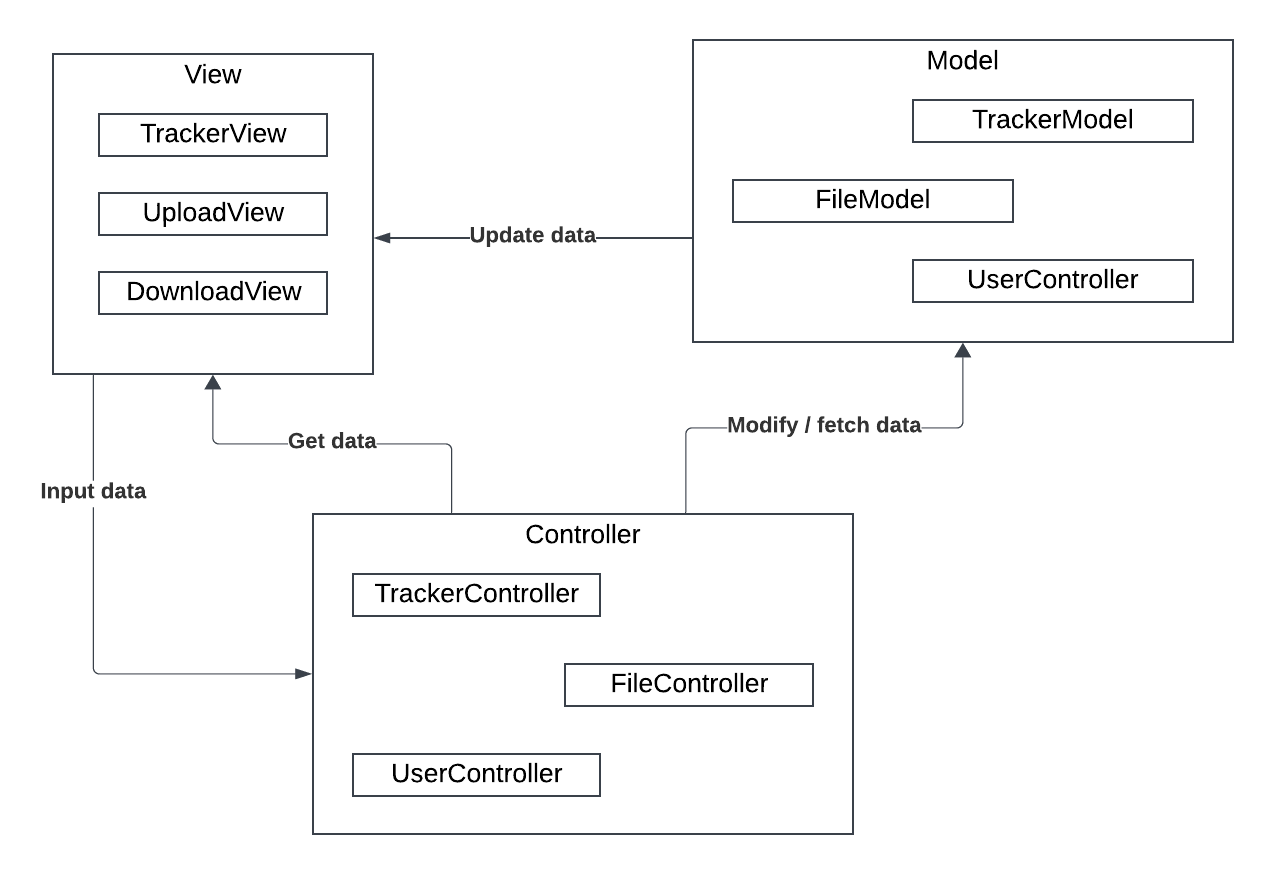
\includegraphics[width=1\textwidth]{MVC.png}
    \captionsetup{labelformat=empty}
    \caption{MVC}
    \label{fig:mvc}
\end{figure}

\textbf{Flow chart của các module:}

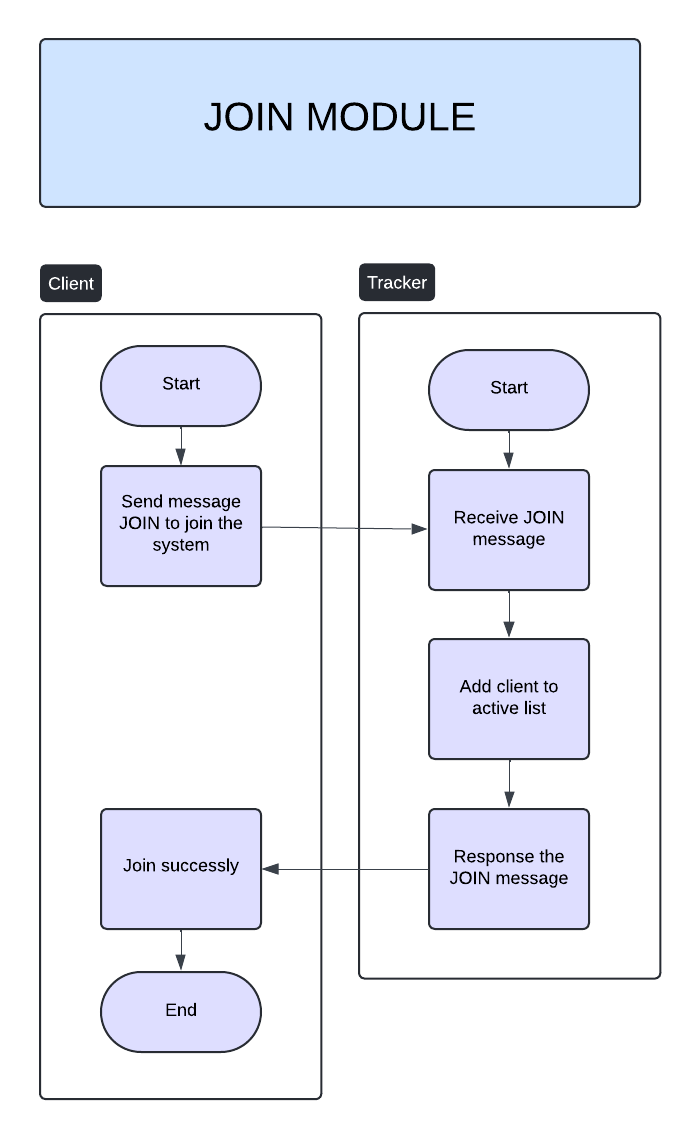
\includegraphics[width=0.5\textwidth]{join_module.png} 

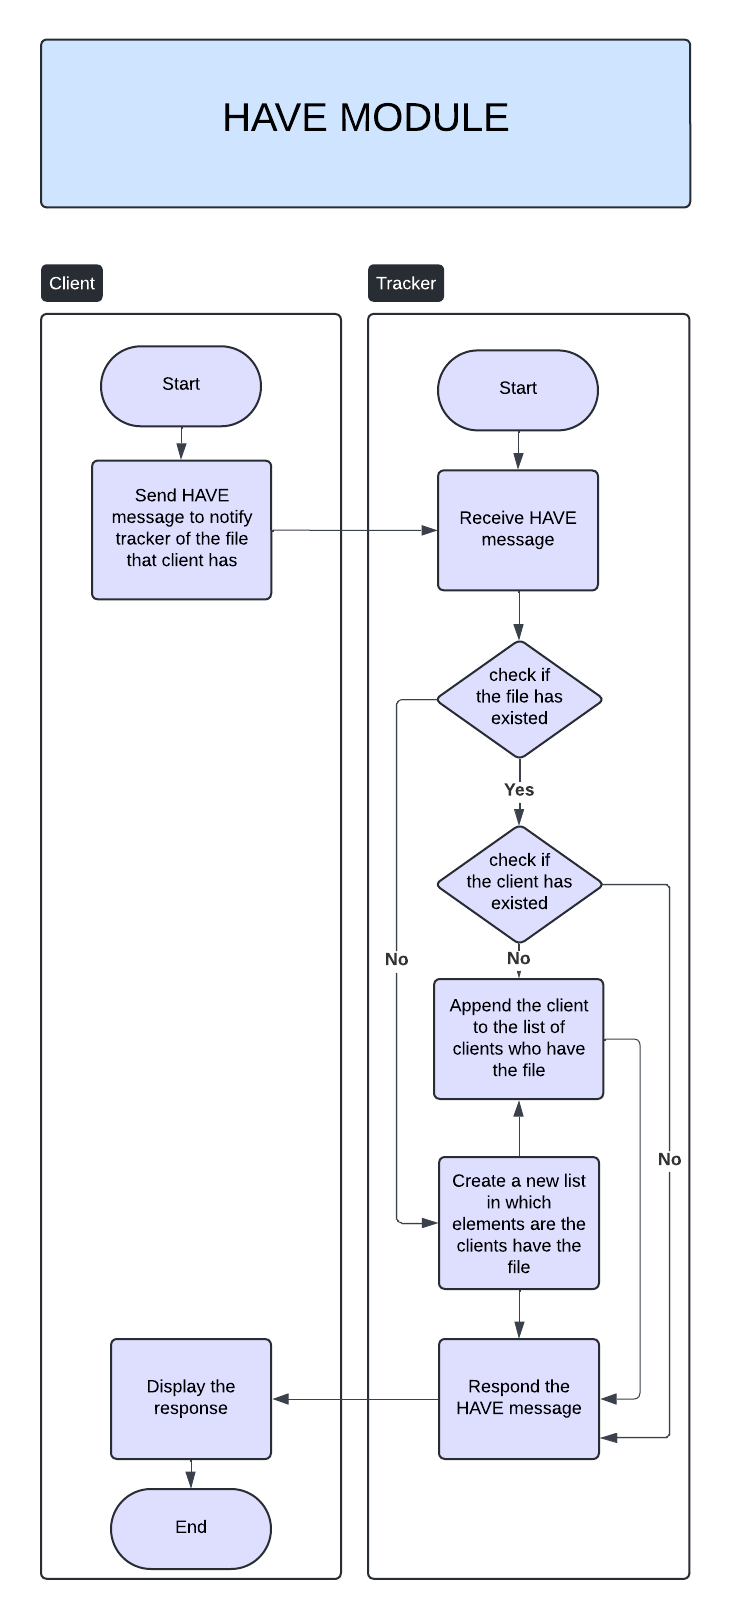
\includegraphics[width=0.5\textwidth]{have_module.png} 

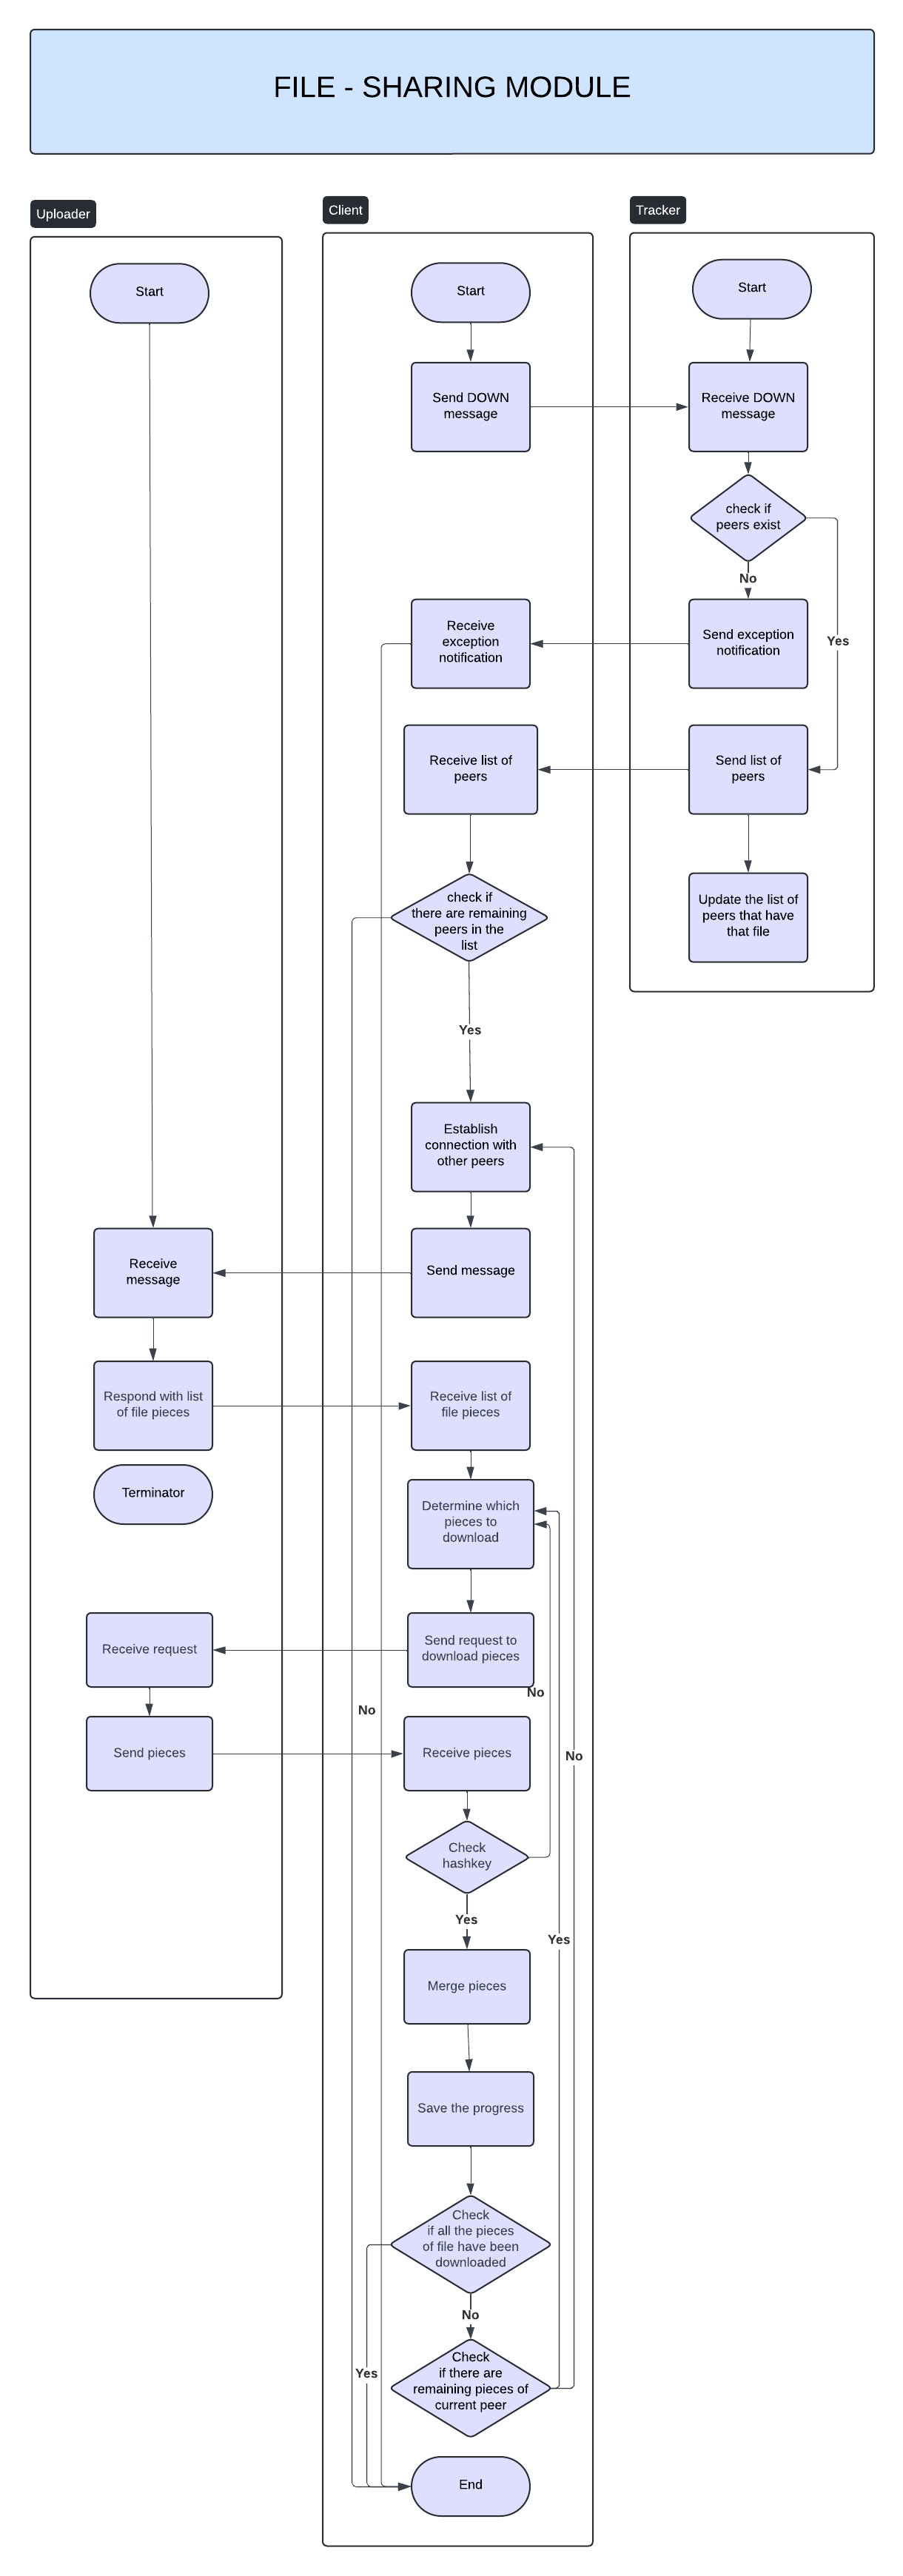
\includegraphics[width=0.5\textwidth]{file_sharing_module.png}

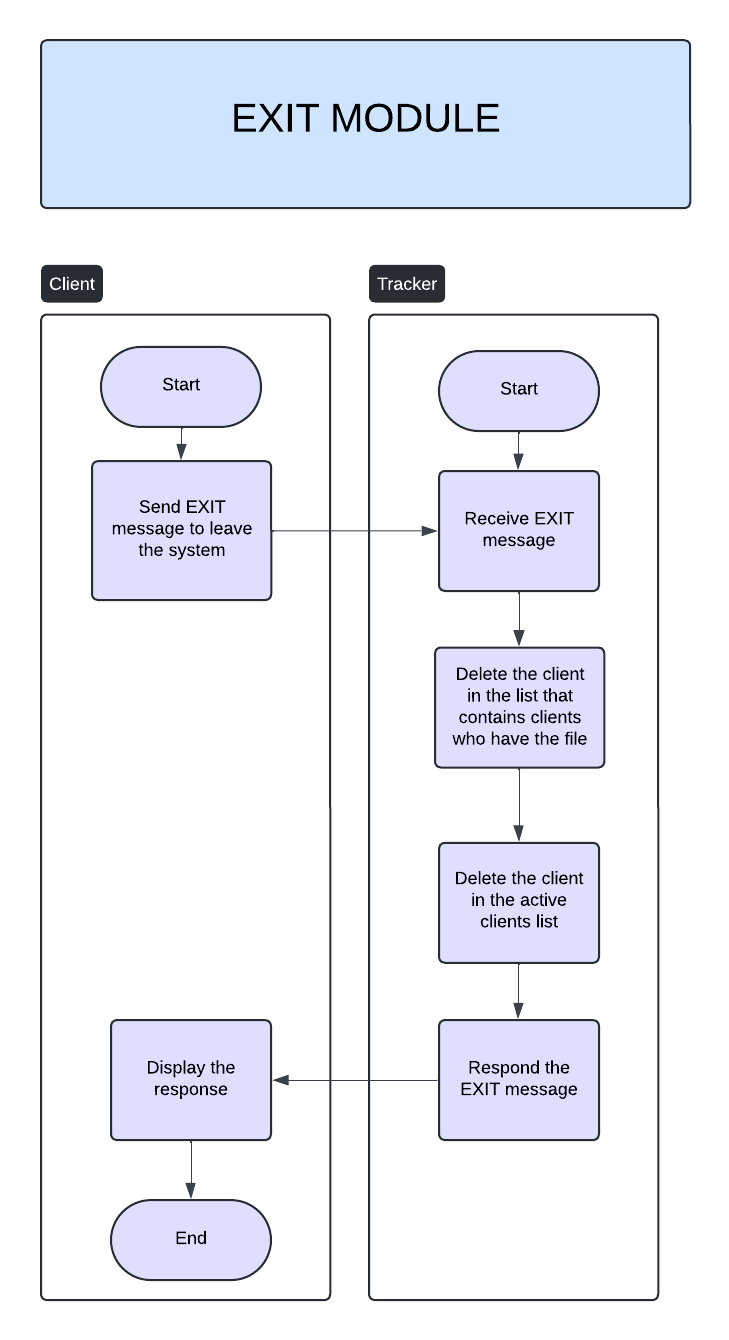
\includegraphics[width=0.5\textwidth]{exit_module.png} 
\newpage

\section{Extra credit}
\subsection{Rarest first}
\begin{figure}[H]
    \centering
    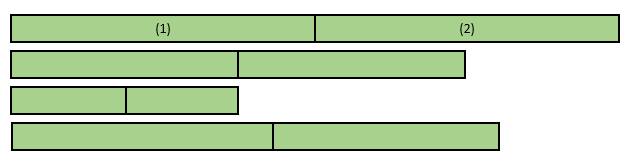
\includegraphics[width=0.9\textwidth]{images/40.png}
    \captionsetup{labelformat=empty}
    % \caption{MVC}
\end{figure}
Để tìm được chunk cần tải, ta sẽ cho vào vòng lặp cho đến khi tìm được chunk cần tải hoặc file đã được tải hết tất cả. \\
Trước khi tìm chunk cần tải, ta sẽ tìm số lượng uploader sở hữu chunk <index> tại thời điểm đang xét:
\begin{figure}[H]
    \centering
    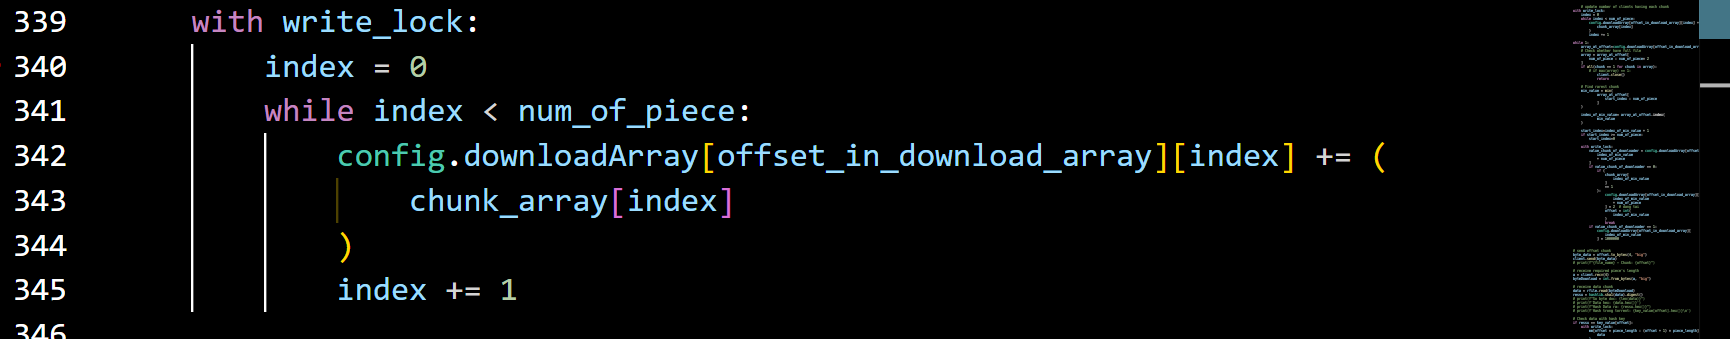
\includegraphics[width=0.9\textwidth]{images/1.png}
    \captionsetup{labelformat=empty}
    % \caption{MVC}
\end{figure}
Tiếp theo, ta sẽ bắt đầu tìm chunk cần tải:
\begin{figure}[H]
    \centering
    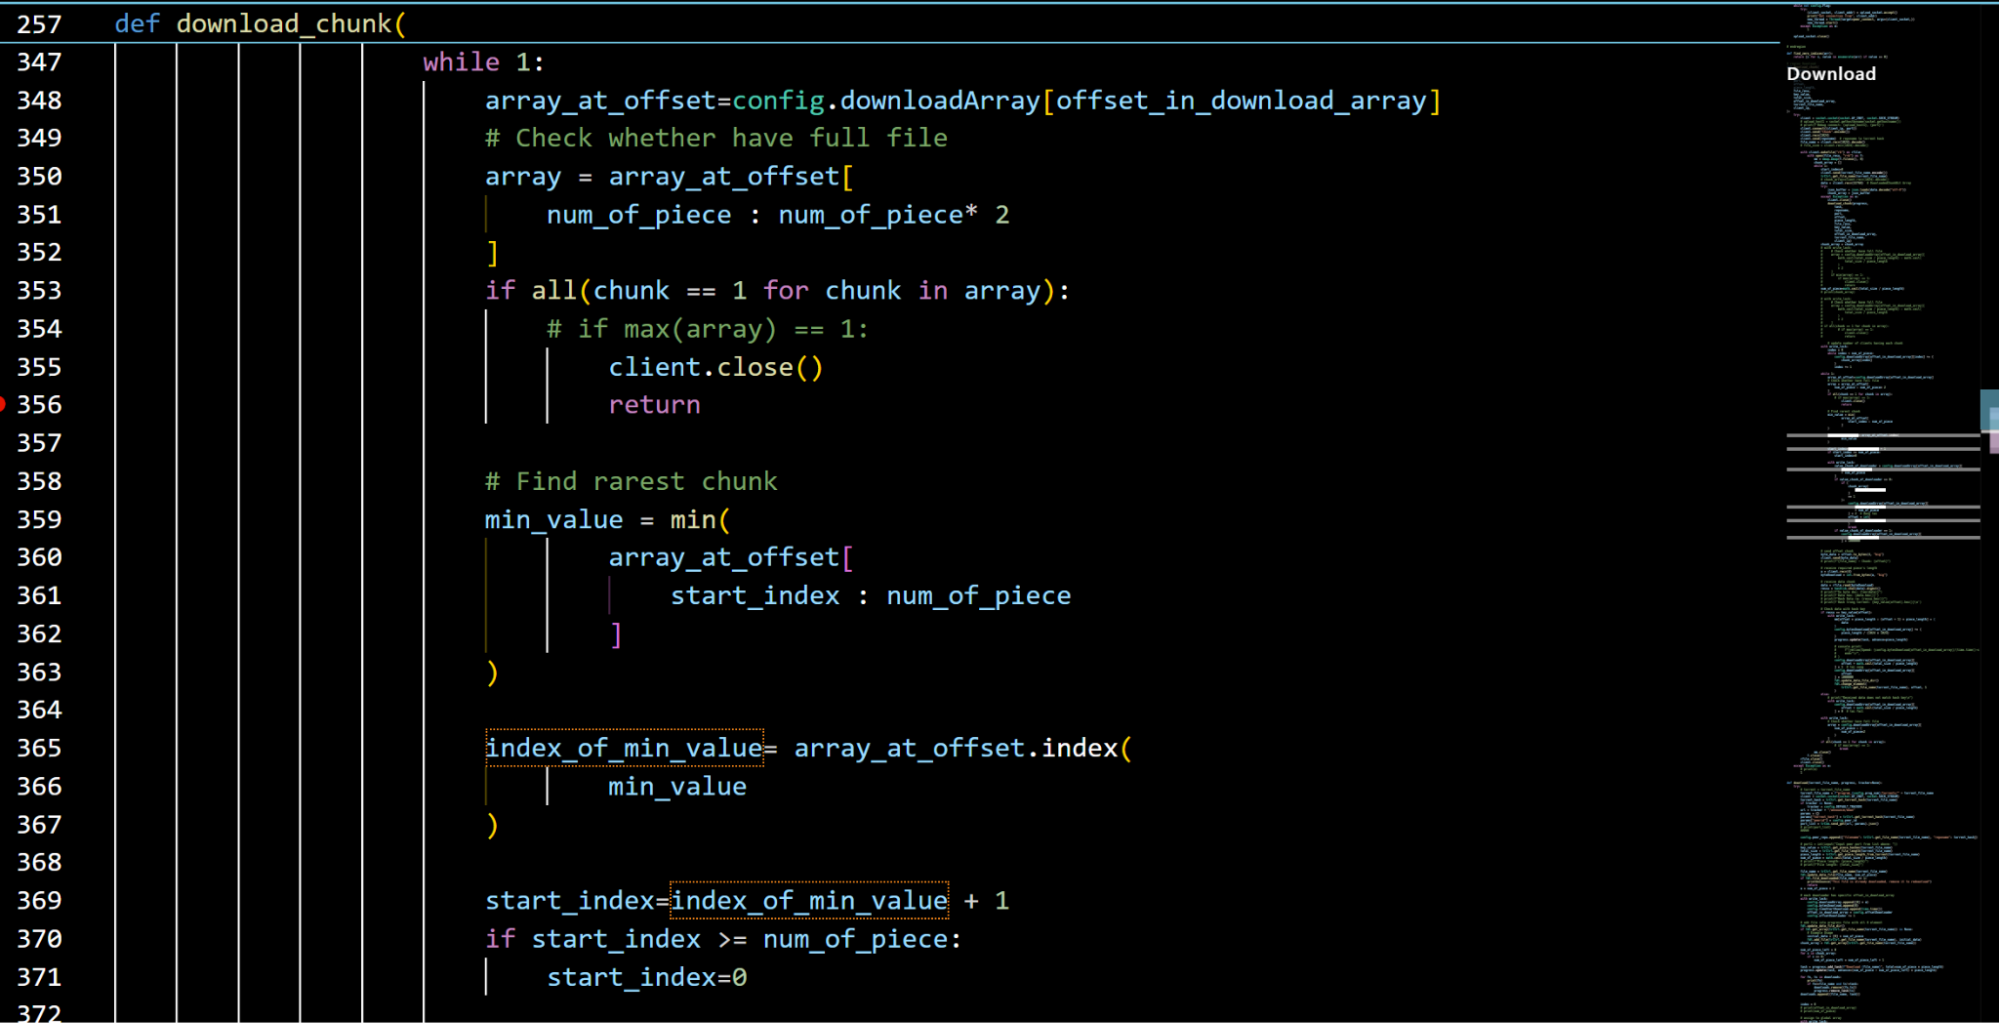
\includegraphics[width=0.9\textwidth]{images/2.png}
    \captionsetup{labelformat=empty}
    % \caption{MVC}
\end{figure}
Ta sẽ có một mảng dynamic 2 chiều (gọi là \texttt{downloadArray}), mỗi phần tử sẽ thuộc về một người tải với một file muốn download xác định (tương ứng với một \texttt{offset\_in\_download\_array}) và có một chiều dài khác nhau ở mỗi phần tử (vì chiều dài phần tử sẽ phụ thuộc vào số lượng chunk của một file). Mỗi phần tử gồm có 2 phần: 

\begin{itemize}
    \item [(1)]:  Ứng với mỗi phần tử trong (1) là số lượng uploader đang có chunk tại index xác định tại thời điểm đang xét (index trong phần (1) cũng chính là số thứ tự của chunk).
    \item [(2)]:  Ứng với mỗi phần tử trong (1), là phần tử trong (2) cách nhau đúng bằng số piece. Ứng với mỗi phần tử trong (2) là tình trạng của chunk:
    \begin{itemize}
        \item 0: chunk này vẫn chưa được tải.
        \item 2: chunk này đang được tải bởi một uploader.
        \item 1: chunk đã được tải xong.
    \end{itemize}
    \item[$\rightarrow$] Chiều dài của phần (1) và (2) bằng nhau.
\end{itemize}

\textbf{Bước 1}: Kiểm tra xem phần (2) của mảng đã tải hết file chưa (thể hiện qua việc tất cả các phần tử của (2) đều là 1). \textbf{\textcolor{red}{Nếu rồi thì dừng.}}

\textbf{Bước 2}: Tìm giá trị nhỏ nhất trong phần (1), đồng thời lấy giá trị index của giá trị nhỏ nhất (thứ tự của chunk tại đó có số lượng uploader là ít nhất).

\textbf{Bước 3}: Trong trường hợp giá trị nhỏ nhất tại index này không thỏa điều kiện, ta sẽ tiếp tục tìm giá trị nhỏ nhất từ vị trí này trở đi. Nếu vị trí mới bắt đầu tìm kiếm này lớn hơn độ dài phần (1), ta sẽ quay về đầu phần (1) để kiếm.
\begin{figure}[H]
    \centering
    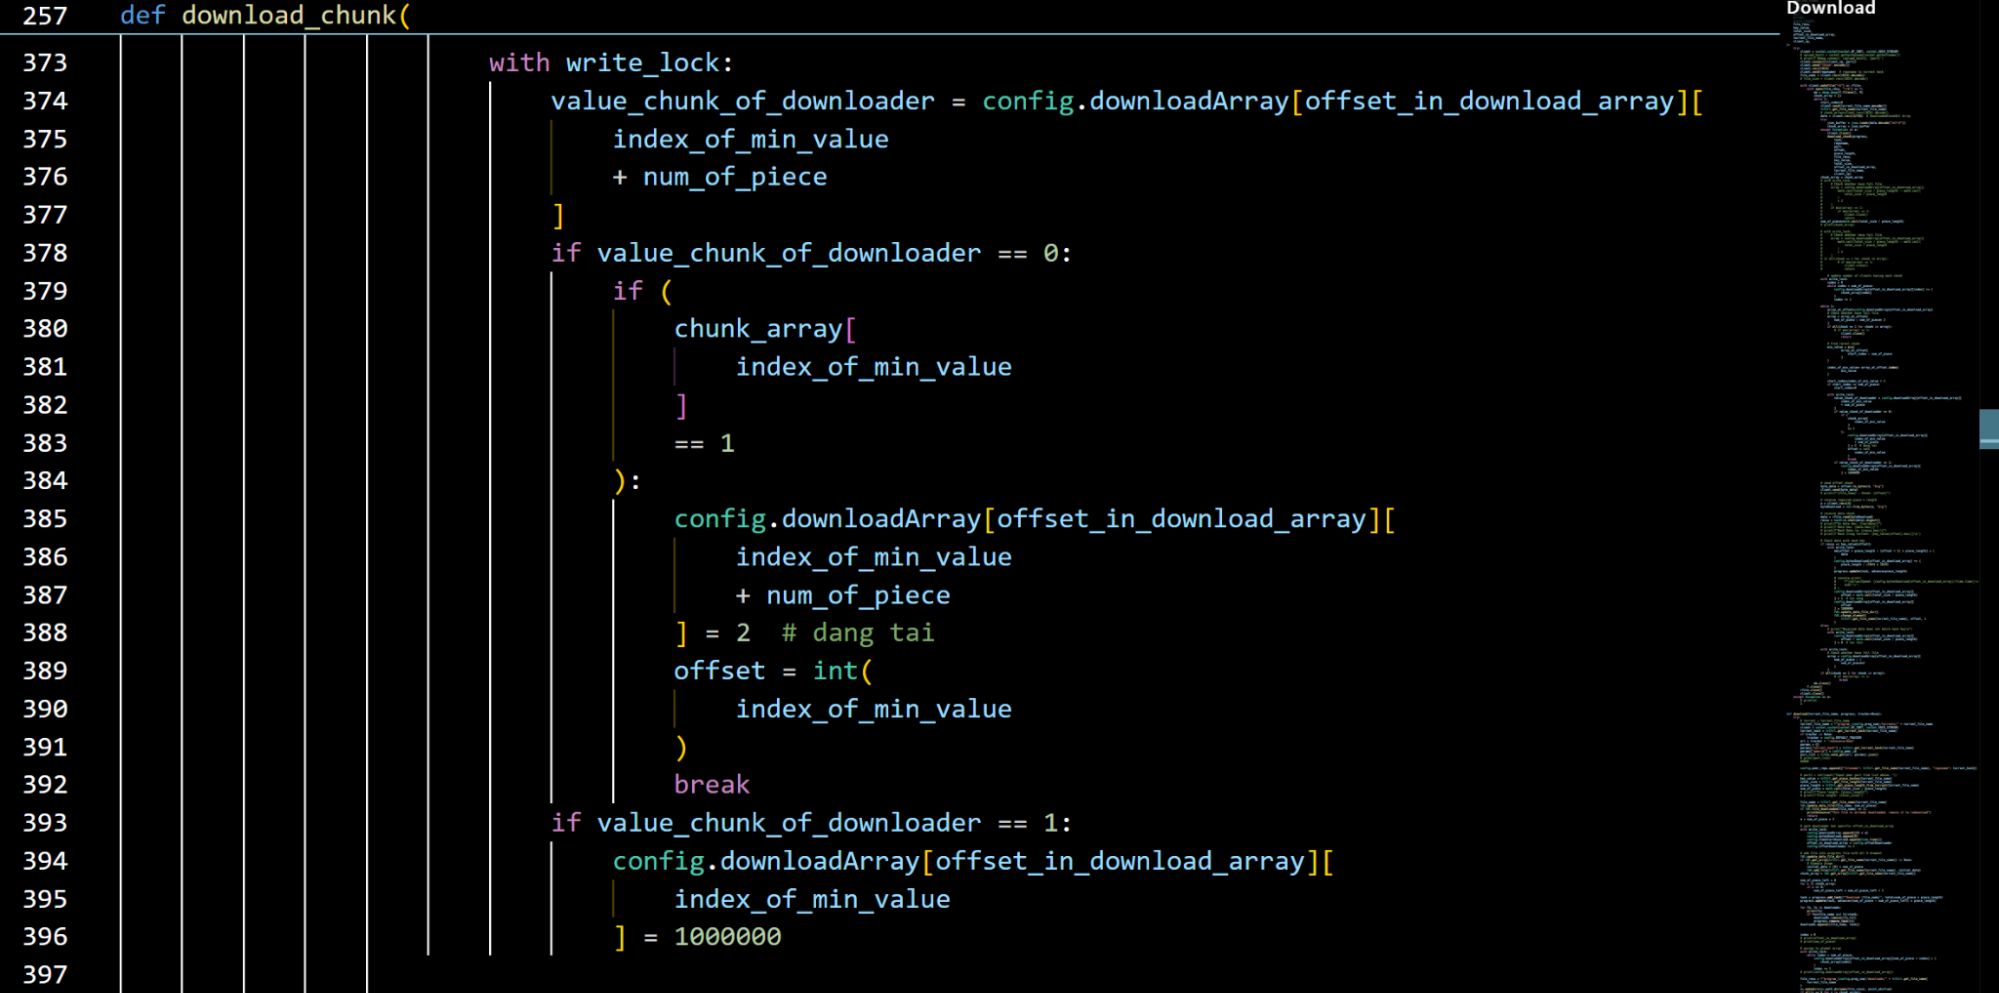
\includegraphics[width=1\textwidth]{images/3.png}
    \captionsetup{labelformat=empty}
    % \caption{MVC}
\end{figure}
\textbf{Bước 4}: Ta sẽ xét giá trị \texttt{index} của \texttt{min\_value} trong phần (1) xem chunk này đã được tải chưa, cũng như uploader có chunk này chưa. Các bước thực hiện như sau:
\begin{itemize}
    \item Nếu thỏa mãn điều kiện, ta sẽ:
    \begin{itemize}
        \item Đánh dấu chunk này đang được tải (gán giá trị \textbf{2}) trong phần (2) ứng với \texttt{index} này.
        \item Trả về \texttt{offset} (thứ tự của chunk cần tải) là \texttt{index} của \texttt{min\_value}.
    \end{itemize}
    \item Nếu chunk tại \texttt{index} này trong phần (2) có giá trị là \textbf{1}, ta sẽ gán giá trị tương ứng của phần (1) thành một giá trị lớn, để tiếp tục tìm \texttt{index} có \texttt{min\_value} khác.
    \item Nếu chunk tại \texttt{index} này trong phần (2) có giá trị là \textbf{2} hoặc \textbf{1}, ta sẽ quay lại tìm \texttt{min\_value} khác.
\end{itemize}

\subsection{Tắt đi tải lại vẫn tiếp tục tải tiếp}
\textit{Ứng với mỗi client sẽ có các xử lý sau:}
\begin{itemize}
    \item \texttt{data\_file.txt}: File này ghi lại toàn bộ tình trạng chunk của tất cả các file của một client xác định.
    \item Trong lúc tải, dữ liệu cũng sẽ được lưu xuống đĩa.
\end{itemize}

\textbf{Khi người dùng tắt và muốn tải lại, thực hiện các bước sau:}
\begin{itemize}
    \item Kiểm tra \texttt{data\_file.txt} xem tất cả các chunk đã tải xong hết chưa để thông báo cho người dùng.
    \item Nếu chưa tải xong, thực hiện:
    \begin{itemize}
        \item Tiếp tục xét \texttt{data\_file.txt} để chọn rarest chunk nhằm yêu cầu uploader tải.
        \item Mở file đã được tải xuống một phần để tiếp tục ghi thêm dữ liệu.
    \end{itemize}
\end{itemize}

\subsection{Tracker Scrape}
\begin{itemize}
    \item Client dùng lệnh \texttt{have file}, lệnh này sẽ kiểm tra và gửi \texttt{announce} thích hợp cho tracker:
    \begin{itemize}
        \item \texttt{have}: Gửi khi file cần tải chưa được tải/ chưa được tải hết.
        \item \texttt{done}: Gửi khi file đã được tải hoàn toàn. Ngoài ra, sau khi tải file xong, client cũng sẽ gửi lệnh \texttt{done}.
    \end{itemize}
    \item Tracker sẽ thực hiện các bước sau:
    \begin{itemize}
        \item Lưu danh sách client theo từng file ứng với lệnh mà client đã gửi.
        \item Khi nhận lệnh \texttt{scrape}, tracker sẽ trả về:
        \begin{itemize}
            \item Số lượng client đã gửi lệnh \texttt{done} (\textit{seeder}).
            \item Số lượng client đã gửi lệnh \texttt{have} (\textit{leecher}).
        \end{itemize}
    \end{itemize}
\end{itemize}

\subsection{Progress Bar}
\begin{itemize}
    \item Khi người dùng nhập lệnh \texttt{progress}, các thanh \textit{progress bar} ứng với các file đang tải sẽ hiện lên, và tồn tại cho đến khi người dùng nhấn một phím bất kỳ để quay về chế độ nhập lệnh.
    \item Mỗi \textit{progress bar} bao gồm:
    \begin{itemize}
        \item Tên file.
        \item Thanh tiến trình (\textit{progress bar}).
        \item Dung lượng đã tải trên tổng dung lượng.
        \item Ước tính thời gian còn lại.
    \end{itemize}
    \item Do chương trình có thể tải nhiều file cùng lúc, nhiều \textit{progress bar} sẽ được hiển thị.
    \item Sau khi tải xong một file:
    \begin{itemize}
        \item Thanh \textit{progress} tương ứng sẽ biến mất sau 10 giây để nhường chỗ cho các thanh khác, giúp giao diện dễ xem hơn.
    \end{itemize}
\end{itemize}


\subsection{Lệnh \texttt{status}:}
\begin{itemize}
    \item Dùng để kiểm tra trạng thái của các file torrent, nhằm xác định các file đã tải xong hay chưa.
\end{itemize}


\section{Demo}
\subsection{DOWN}
\begin{itemize}
    \item HELP: Chương trình có lệnh help để xem tổng quan các lệnh có thể sử dụng và khi dùng lệnh help kèm với lệnh khác có thể xem kĩ hơn về 1 lệnh và ví dụ khi sử dụng
\end{itemize}
\begin{figure}[H]
    \centering
    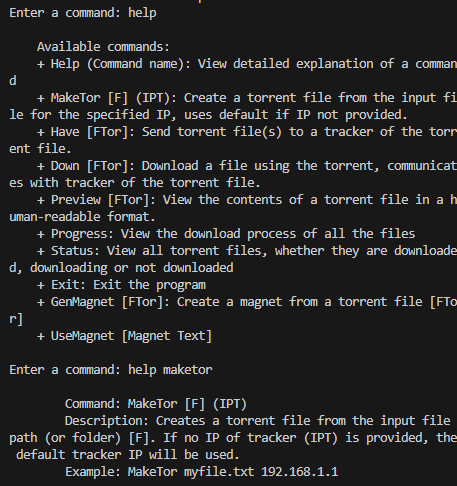
\includegraphics[width=1\textwidth]{images/4.png}
    \captionsetup{labelformat=empty}
    % \caption{MVC}
\end{figure}
\begin{itemize}
    \item maketor: dùng lệnh maketor kèm với tên file để tạo file torrent
\end{itemize}
\begin{figure}[H]
    \centering
    
\includegraphics[width=1\textwidth]{images/5.png}
    \captionsetup{labelformat=empty}
    % \caption{MVC}
\end{figure}
\begin{itemize}
    \item Magnet text:
    \begin{itemize}
        \item Tạo magnet text để các client khác có thể tải file torrent từ magnet text thông qua lệnh genmagnet + tên file torrent
        \item Nhập lệnh usemagnet + magnet text để dùng magnet text tải file torrent
    \end{itemize}
\end{itemize}
\begin{figure}[H]
    \centering
    
\includegraphics[width=1\textwidth]{images/6.png}
    \captionsetup{labelformat=empty}
    % \caption{MVC}
\end{figure}
\begin{figure}[H]
    \centering
    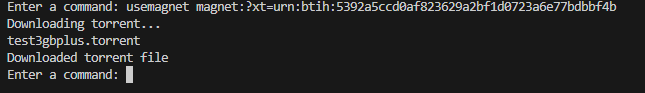
\includegraphics[width=1\textwidth]{images/7.png}
    \captionsetup{labelformat=empty}
    % \caption{MVC}
\end{figure}

\noindent \textbf{CLIENT 2}\\
Client 2 kết nối với tracker và khai báo các file torrent mình đang có với tracker (Client thuộc về “program 2”) và khi vừa vào ta sẽ cho ping tracker để xem tracker còn online không.\\
\begin{figure}[H]
    \centering
    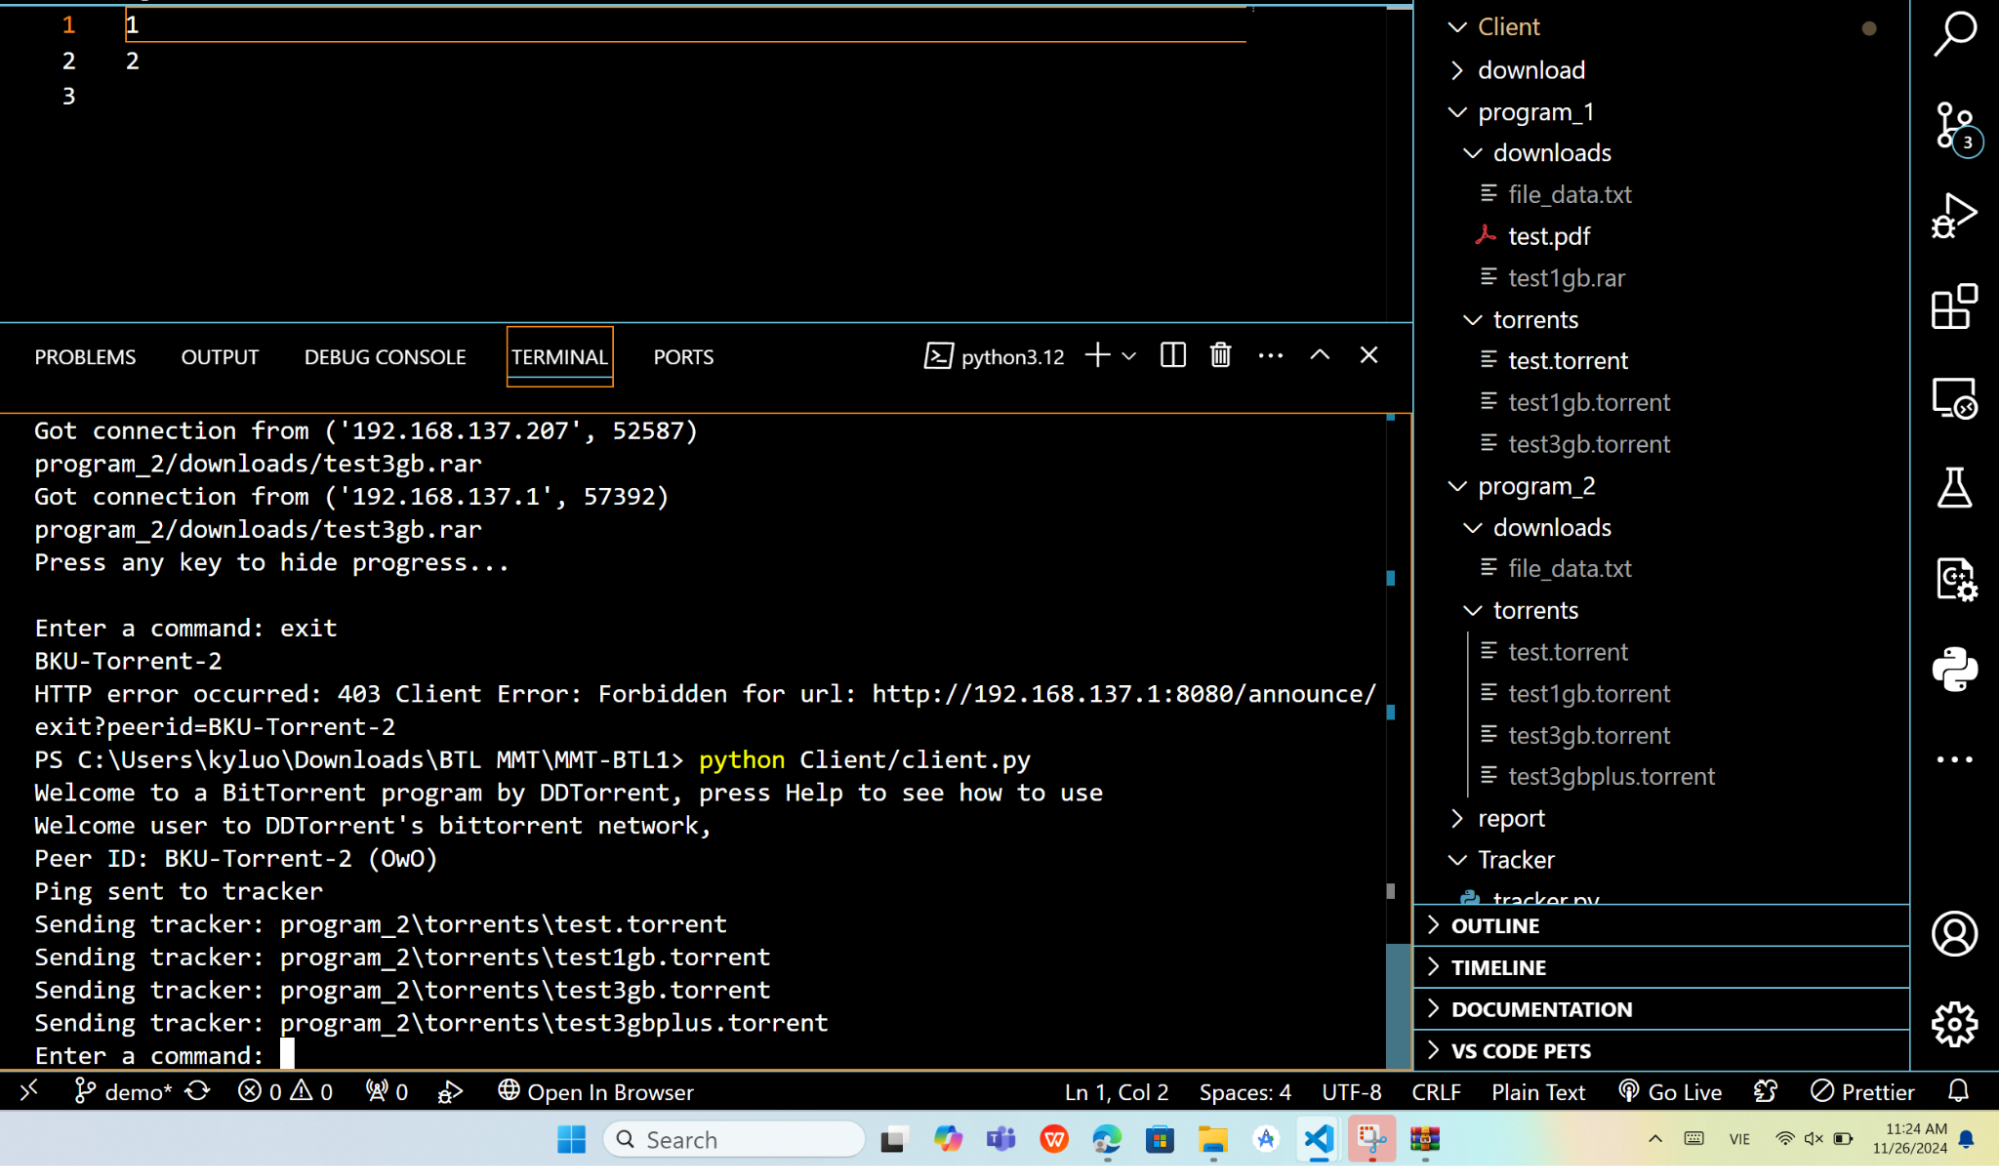
\includegraphics[width=1\textwidth]{images/8.png}
    \captionsetup{labelformat=empty}
    % \caption{MVC}
\end{figure}
\begin{itemize}
    \item Client 1 bắt đầu với nhiệm vũ làm seeder có sẵn hết tất cả file
    \item Tại thời điểm 11:26, client 1 nhận được connection để tải test3gb.rar từ client 2
\end{itemize}
\begin{figure}[H]
    \centering
    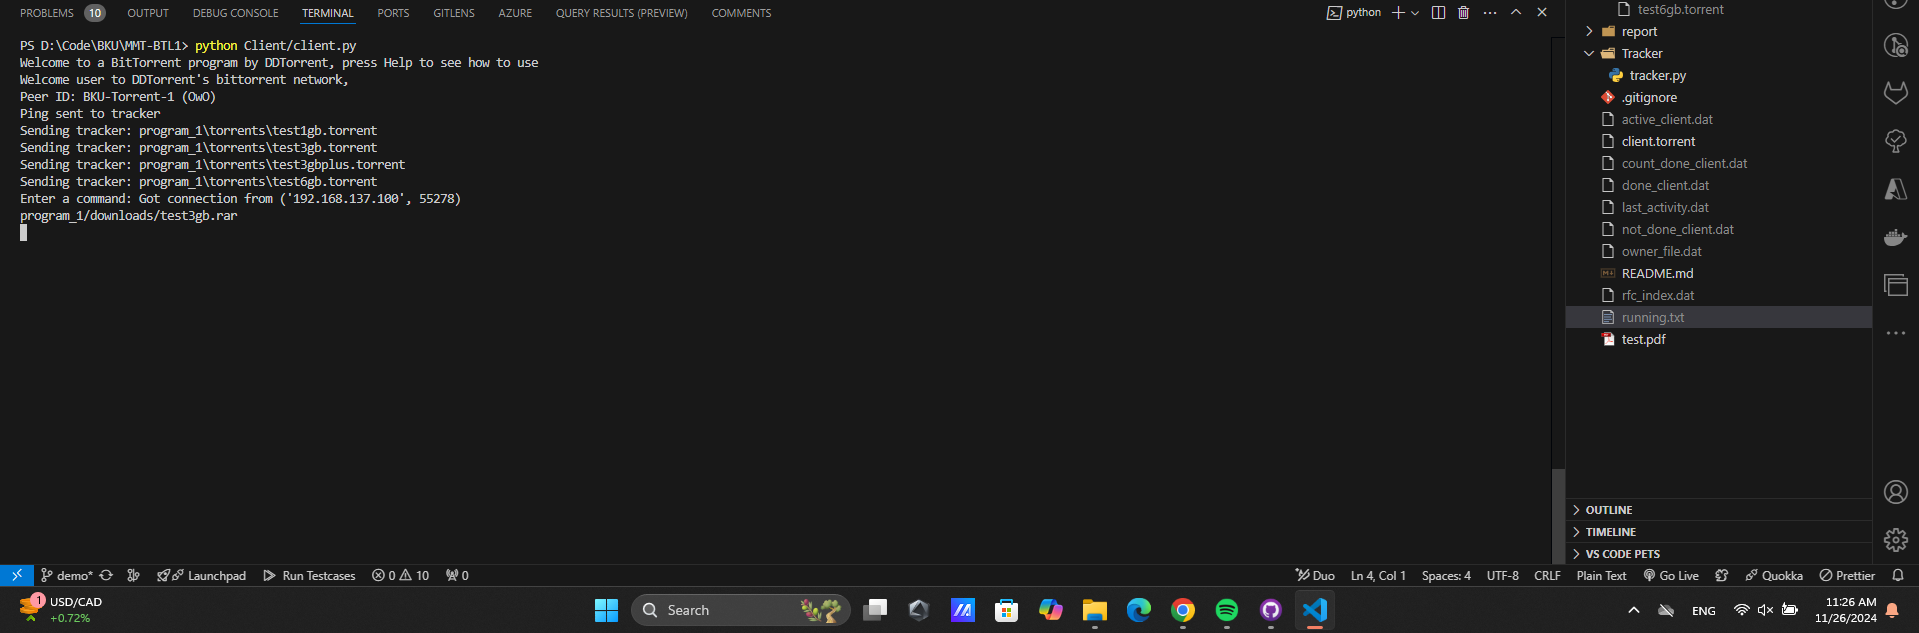
\includegraphics[width=1\textwidth]{images/9.png}
    \captionsetup{labelformat=empty}
    % \caption{MVC}
\end{figure}

Client 2 tiến hành tải test3gb.rar thông qua test3gb.torrent. Lúc này file test3gb.rar sẽ được tạo để ghi dữ liệu cũng như nhập lệnh “progress” để dễ dàng theo dõi.
\begin{figure}[H]
    \centering
    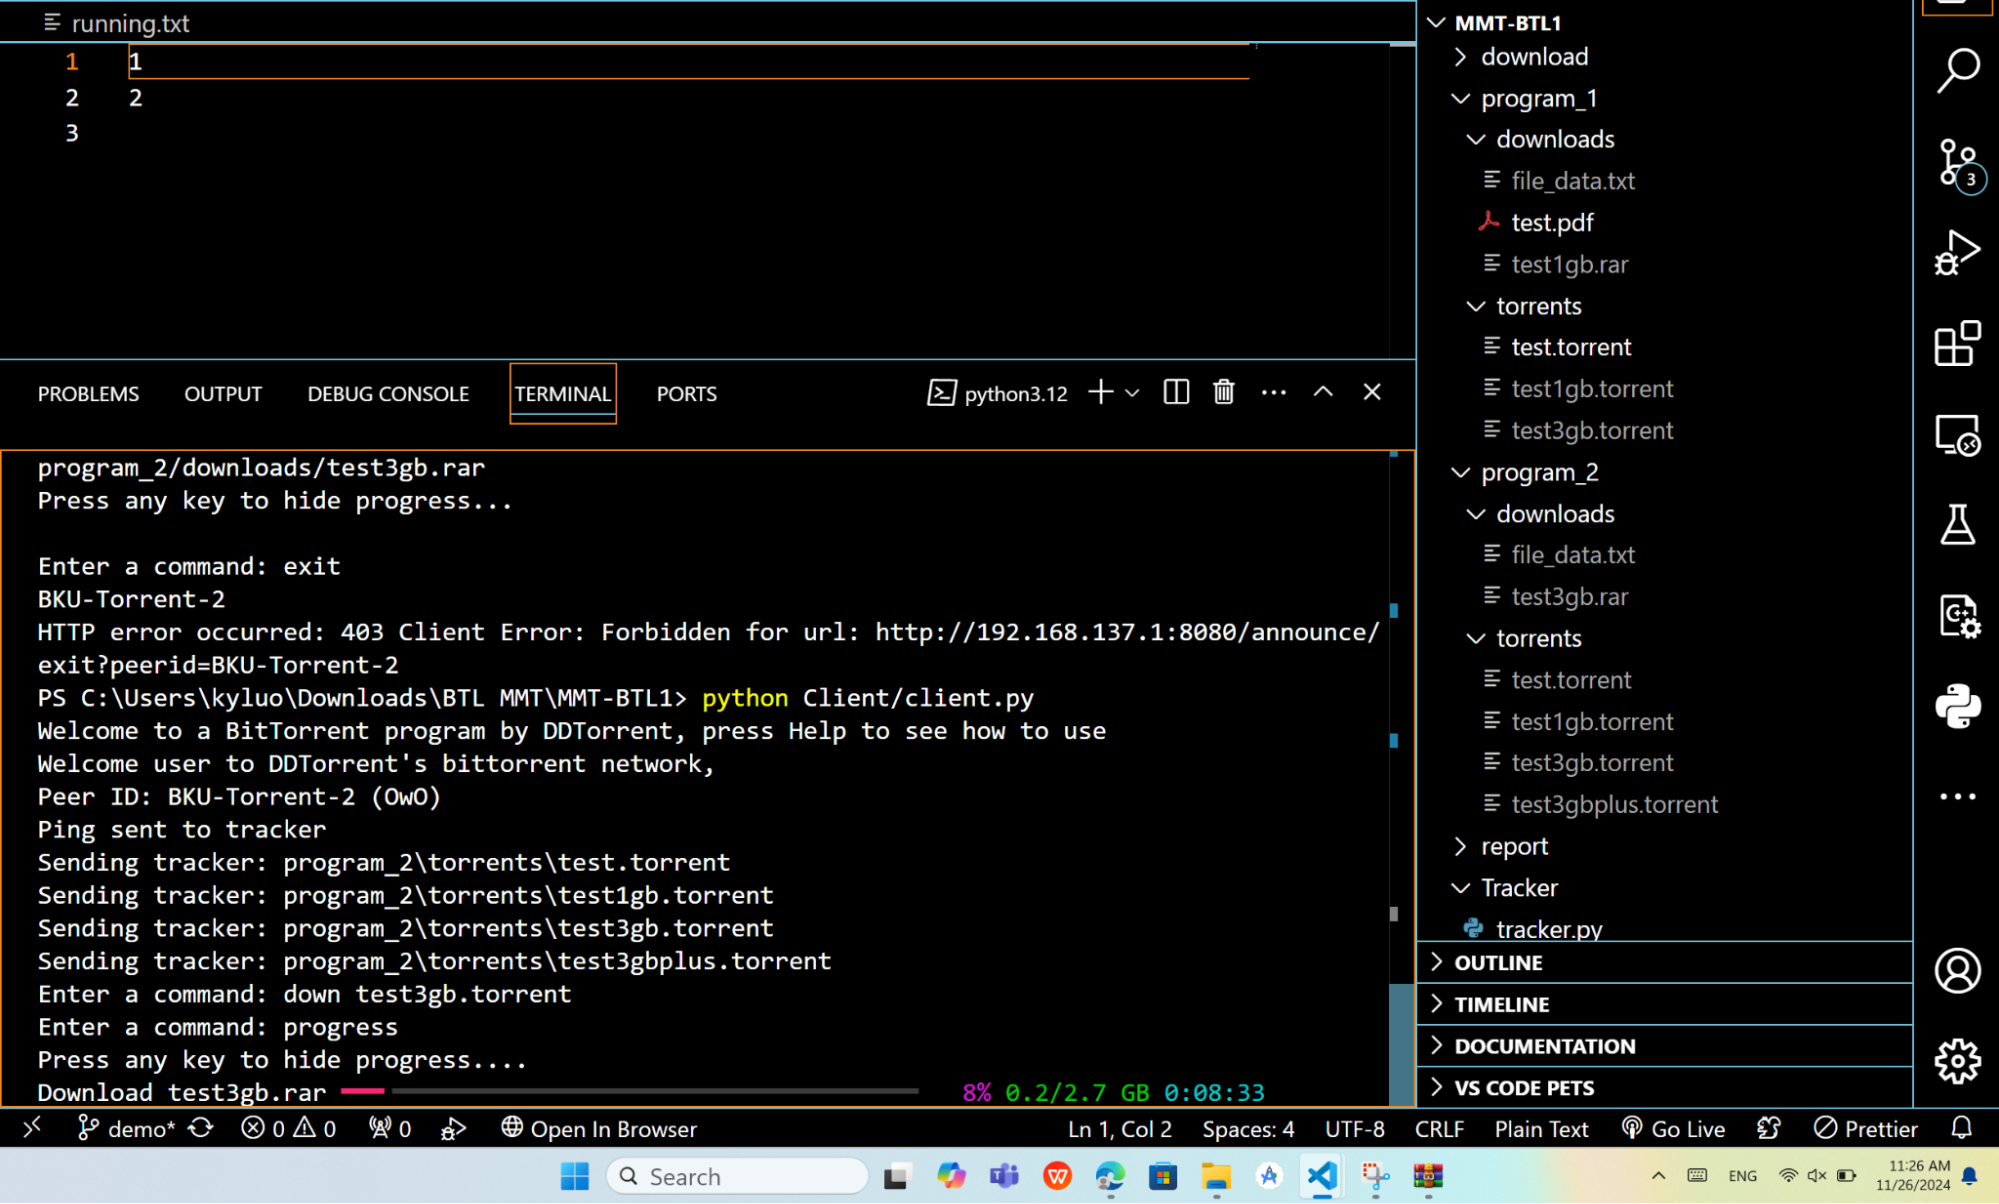
\includegraphics[width=1\textwidth]{images/10.png}
    \captionsetup{labelformat=empty}
    % \caption{MVC}
\end{figure}
Có thể thấy tại thời điểm này file vẫn chưa thể mở được (11:27)
\begin{figure}[H]
    \centering
    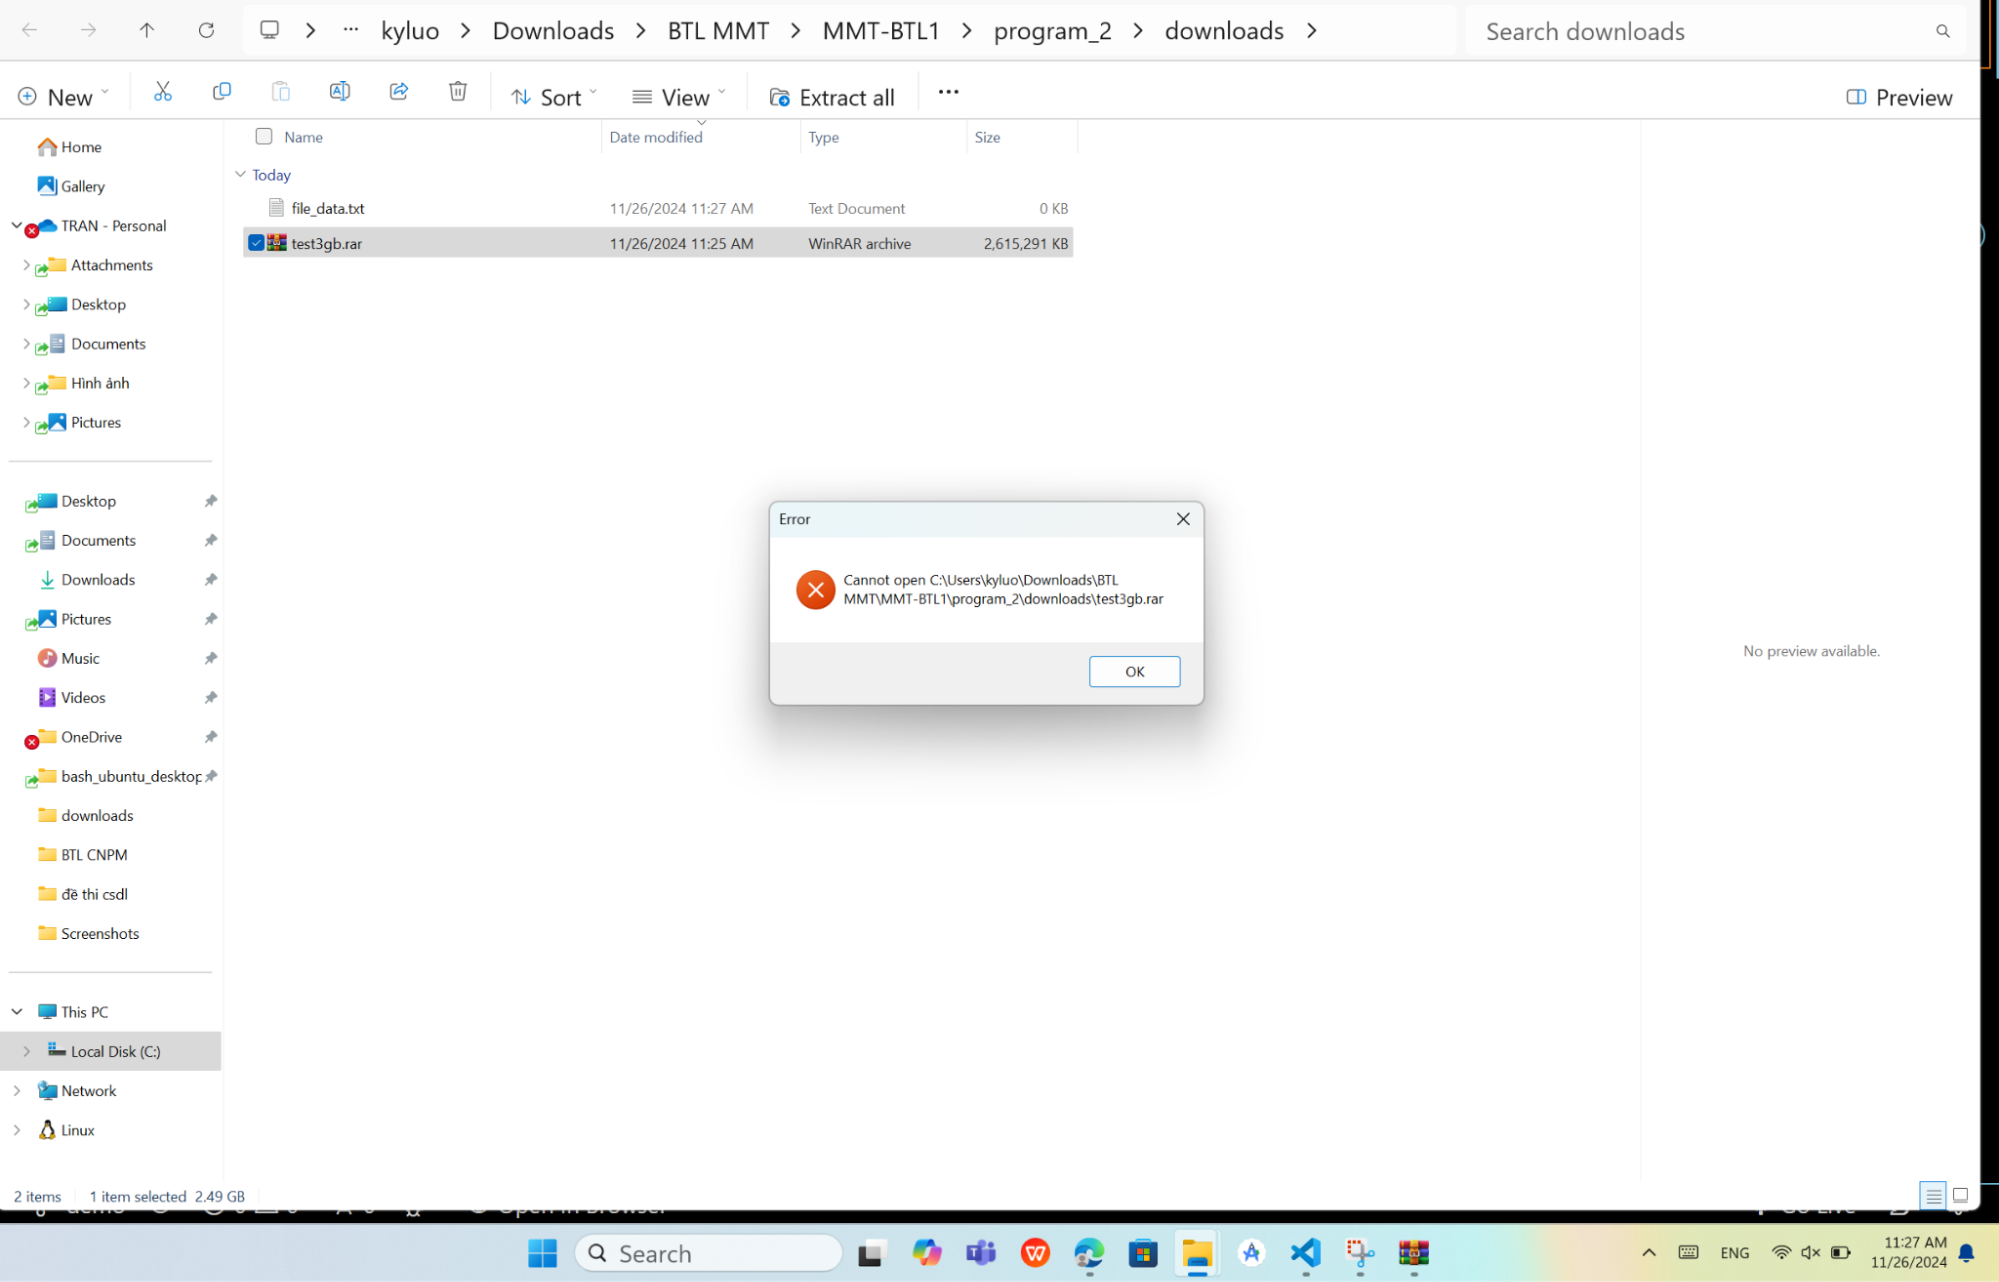
\includegraphics[width=1\textwidth]{images/11.png}
    \captionsetup{labelformat=empty}
    % \caption{MVC}
\end{figure}
Tiếp theo, client 2 sẽ thoát khỏi chương trình, ngắt kết nối(11:28)
\begin{figure}[H]
    \centering
    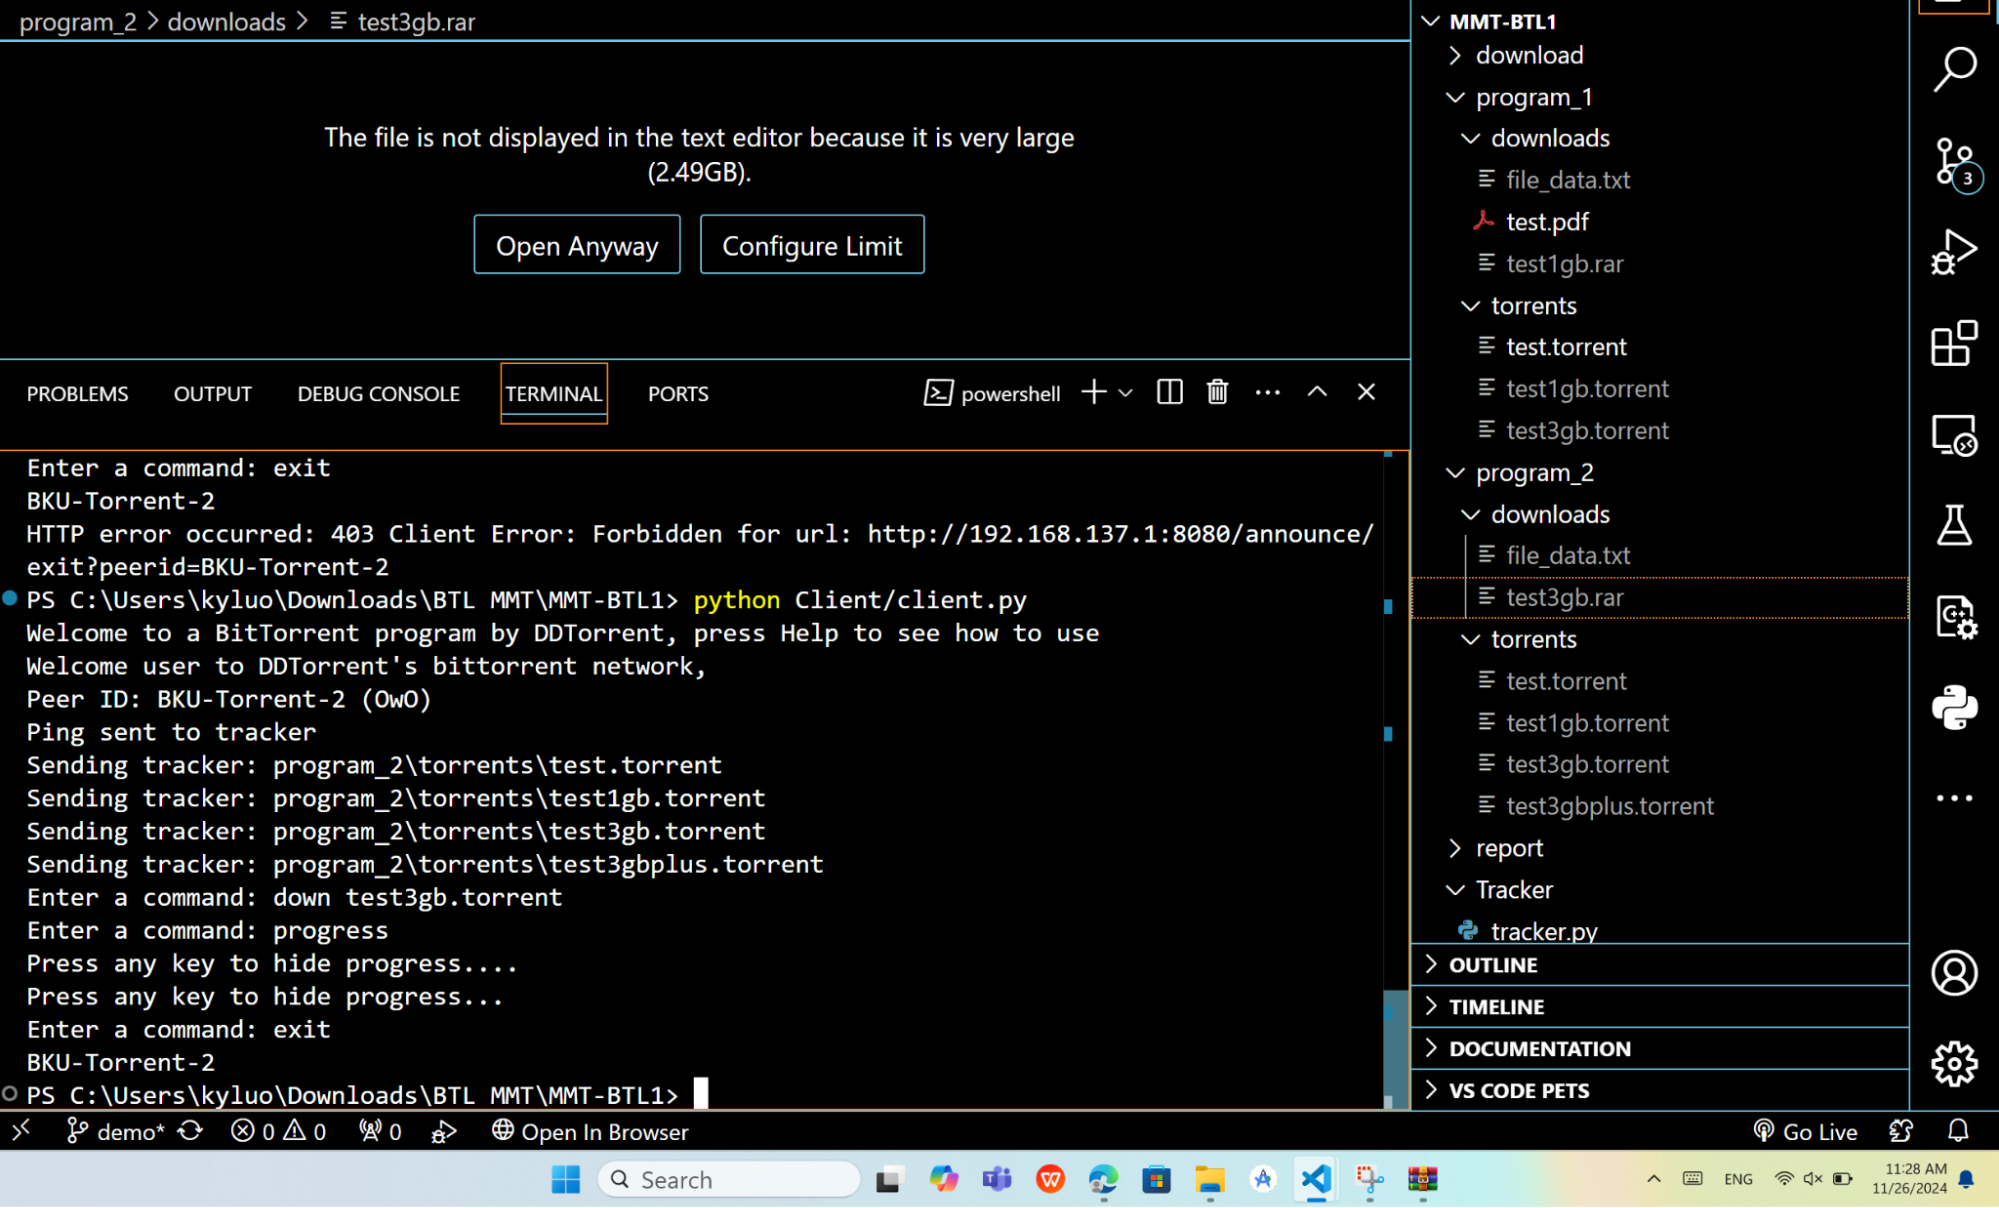
\includegraphics[width=0.8\textwidth]{images/12.png}
    \captionsetup{labelformat=empty}
    % \caption{MVC}
\end{figure}
Sau đó Client quay trở lại, có thể thấy file đang được tải tiếp chứ không quay lại tải từ đầu (11:28)
\begin{figure}[H]
    \centering
    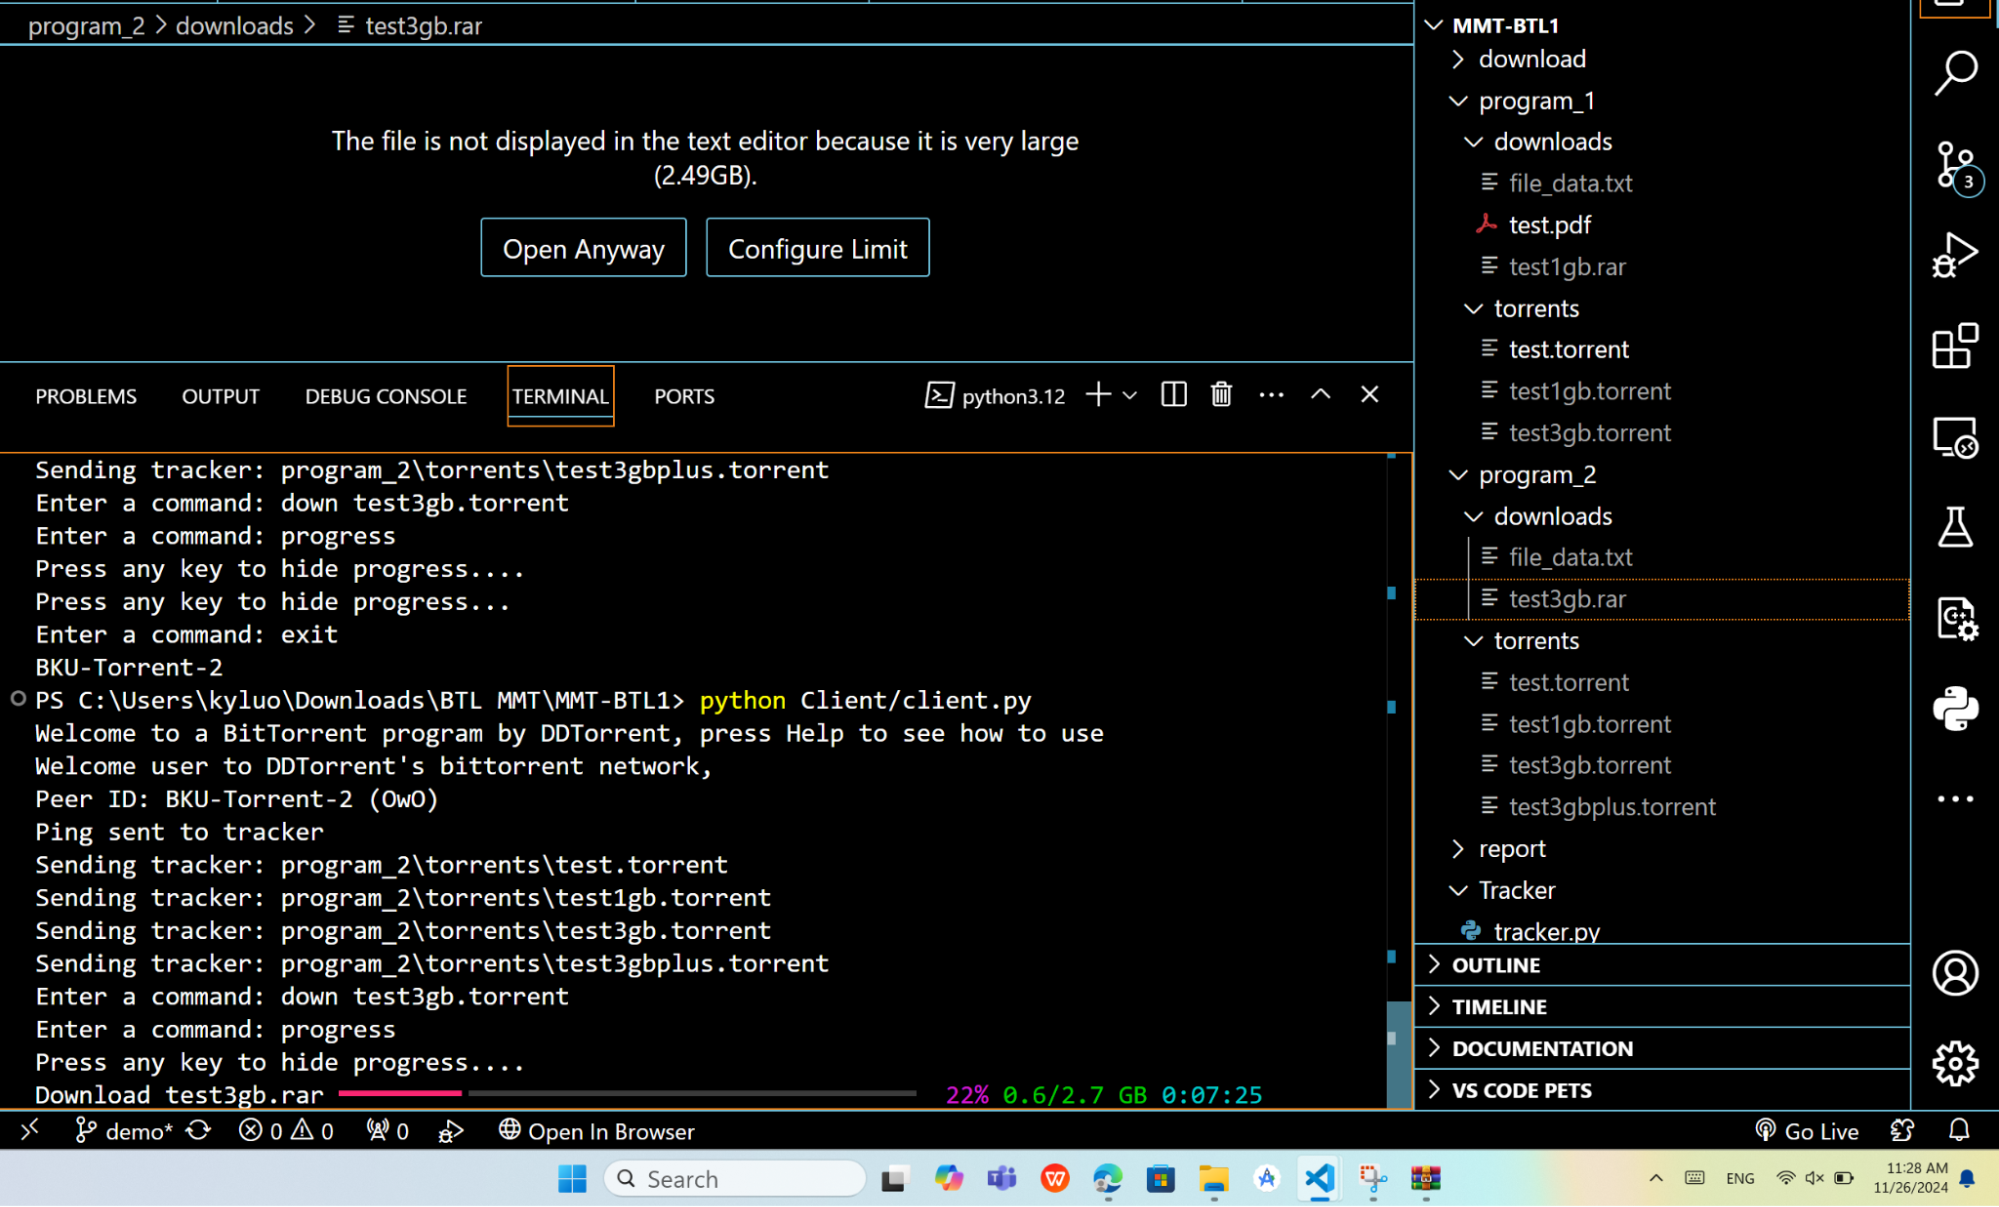
\includegraphics[width=0.8\textwidth]{images/13.png}
    \captionsetup{labelformat=empty}
    % \caption{MVC}
\end{figure}
Lúc này file đã tải xong, đồng thời Client 2 cũng đang kết nối với các Client khác để tải file cho client khác.
\begin{figure}[H]
    \centering
    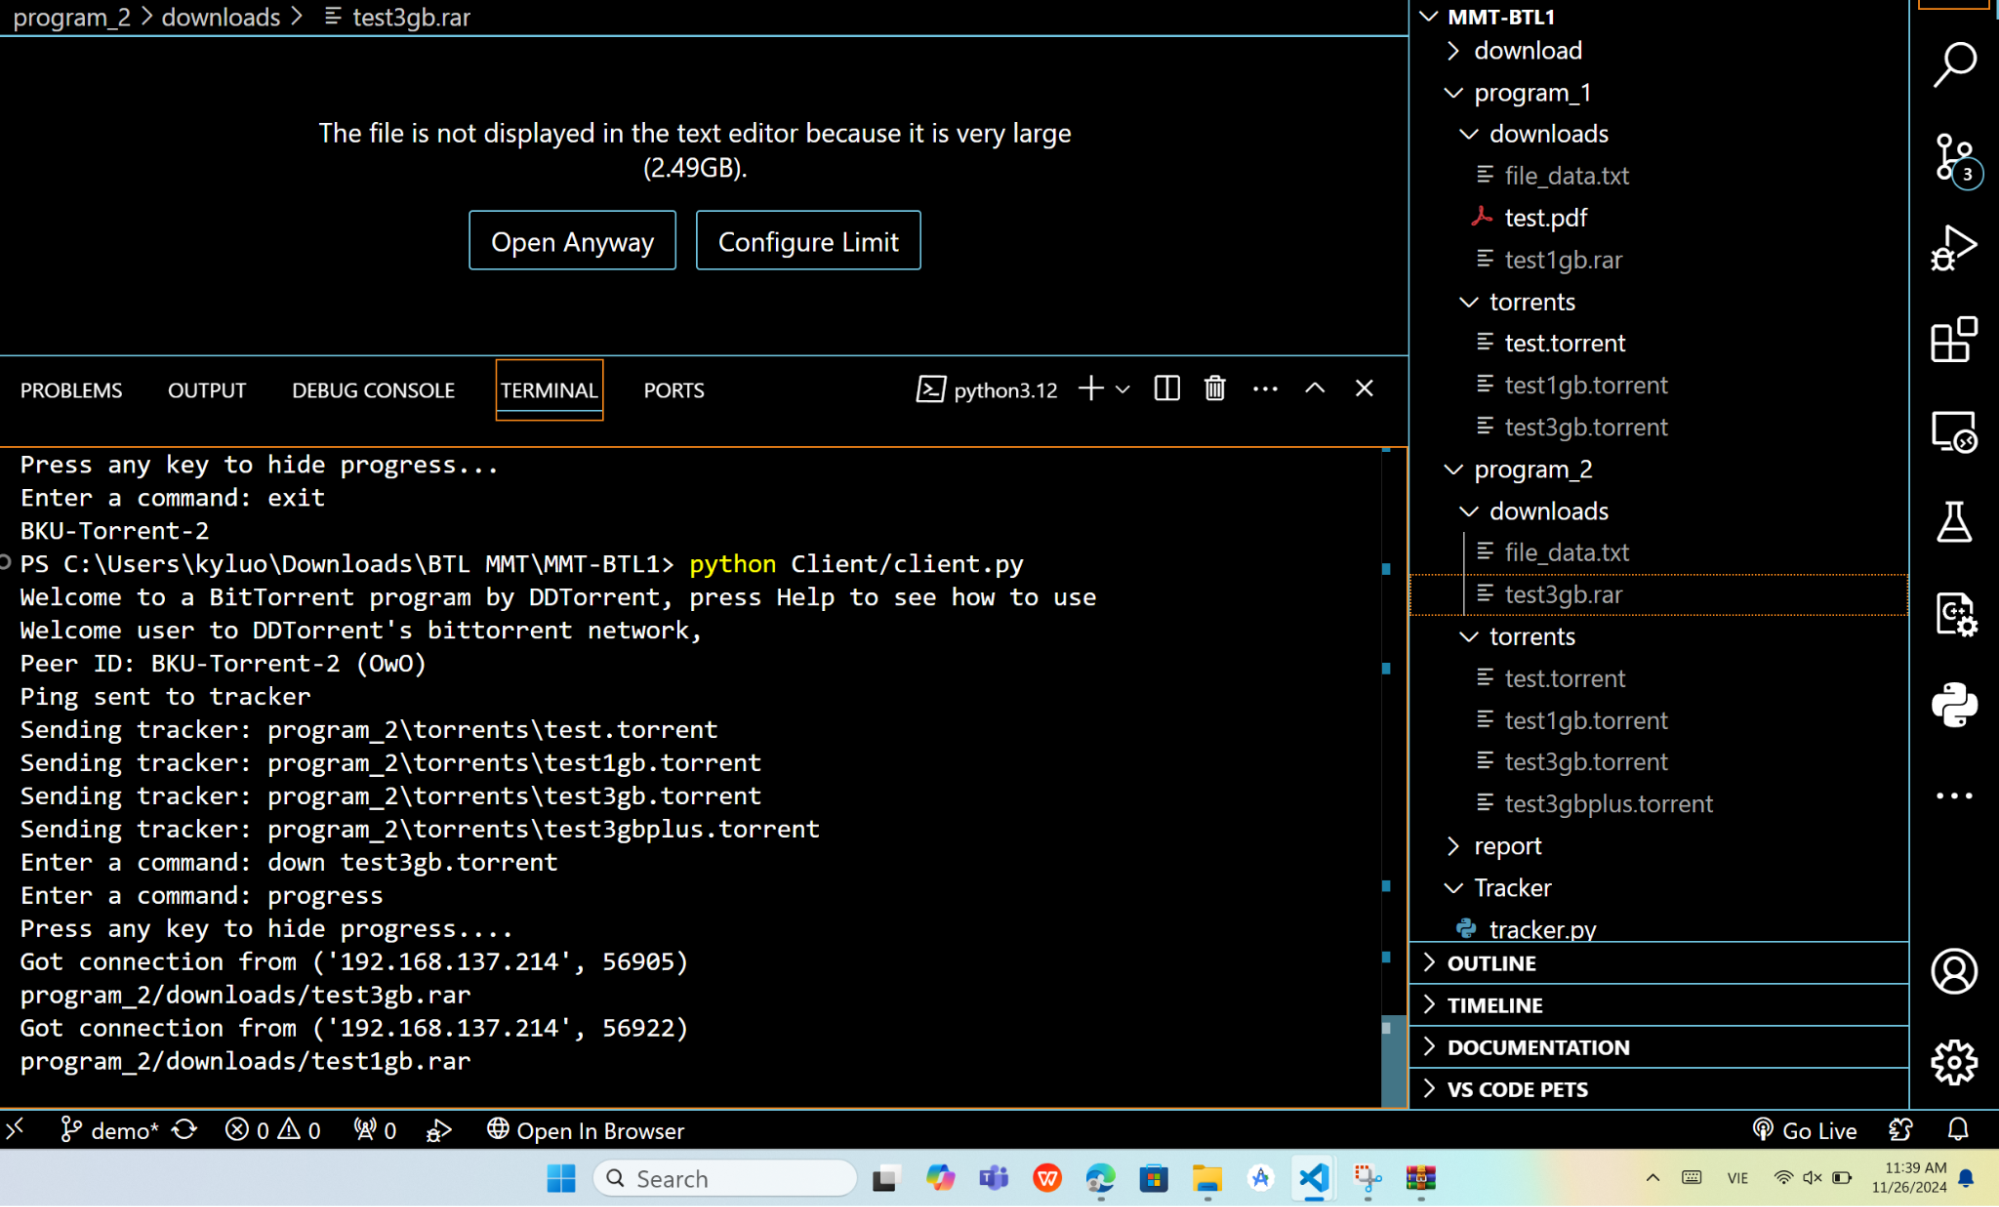
\includegraphics[width=1\textwidth]{images/14.png}
    \captionsetup{labelformat=empty}
    % \caption{MVC}
\end{figure}
Lúc này, vì file đã được tải xong nên đã có thể mở được
\begin{figure}[H]
    \centering
    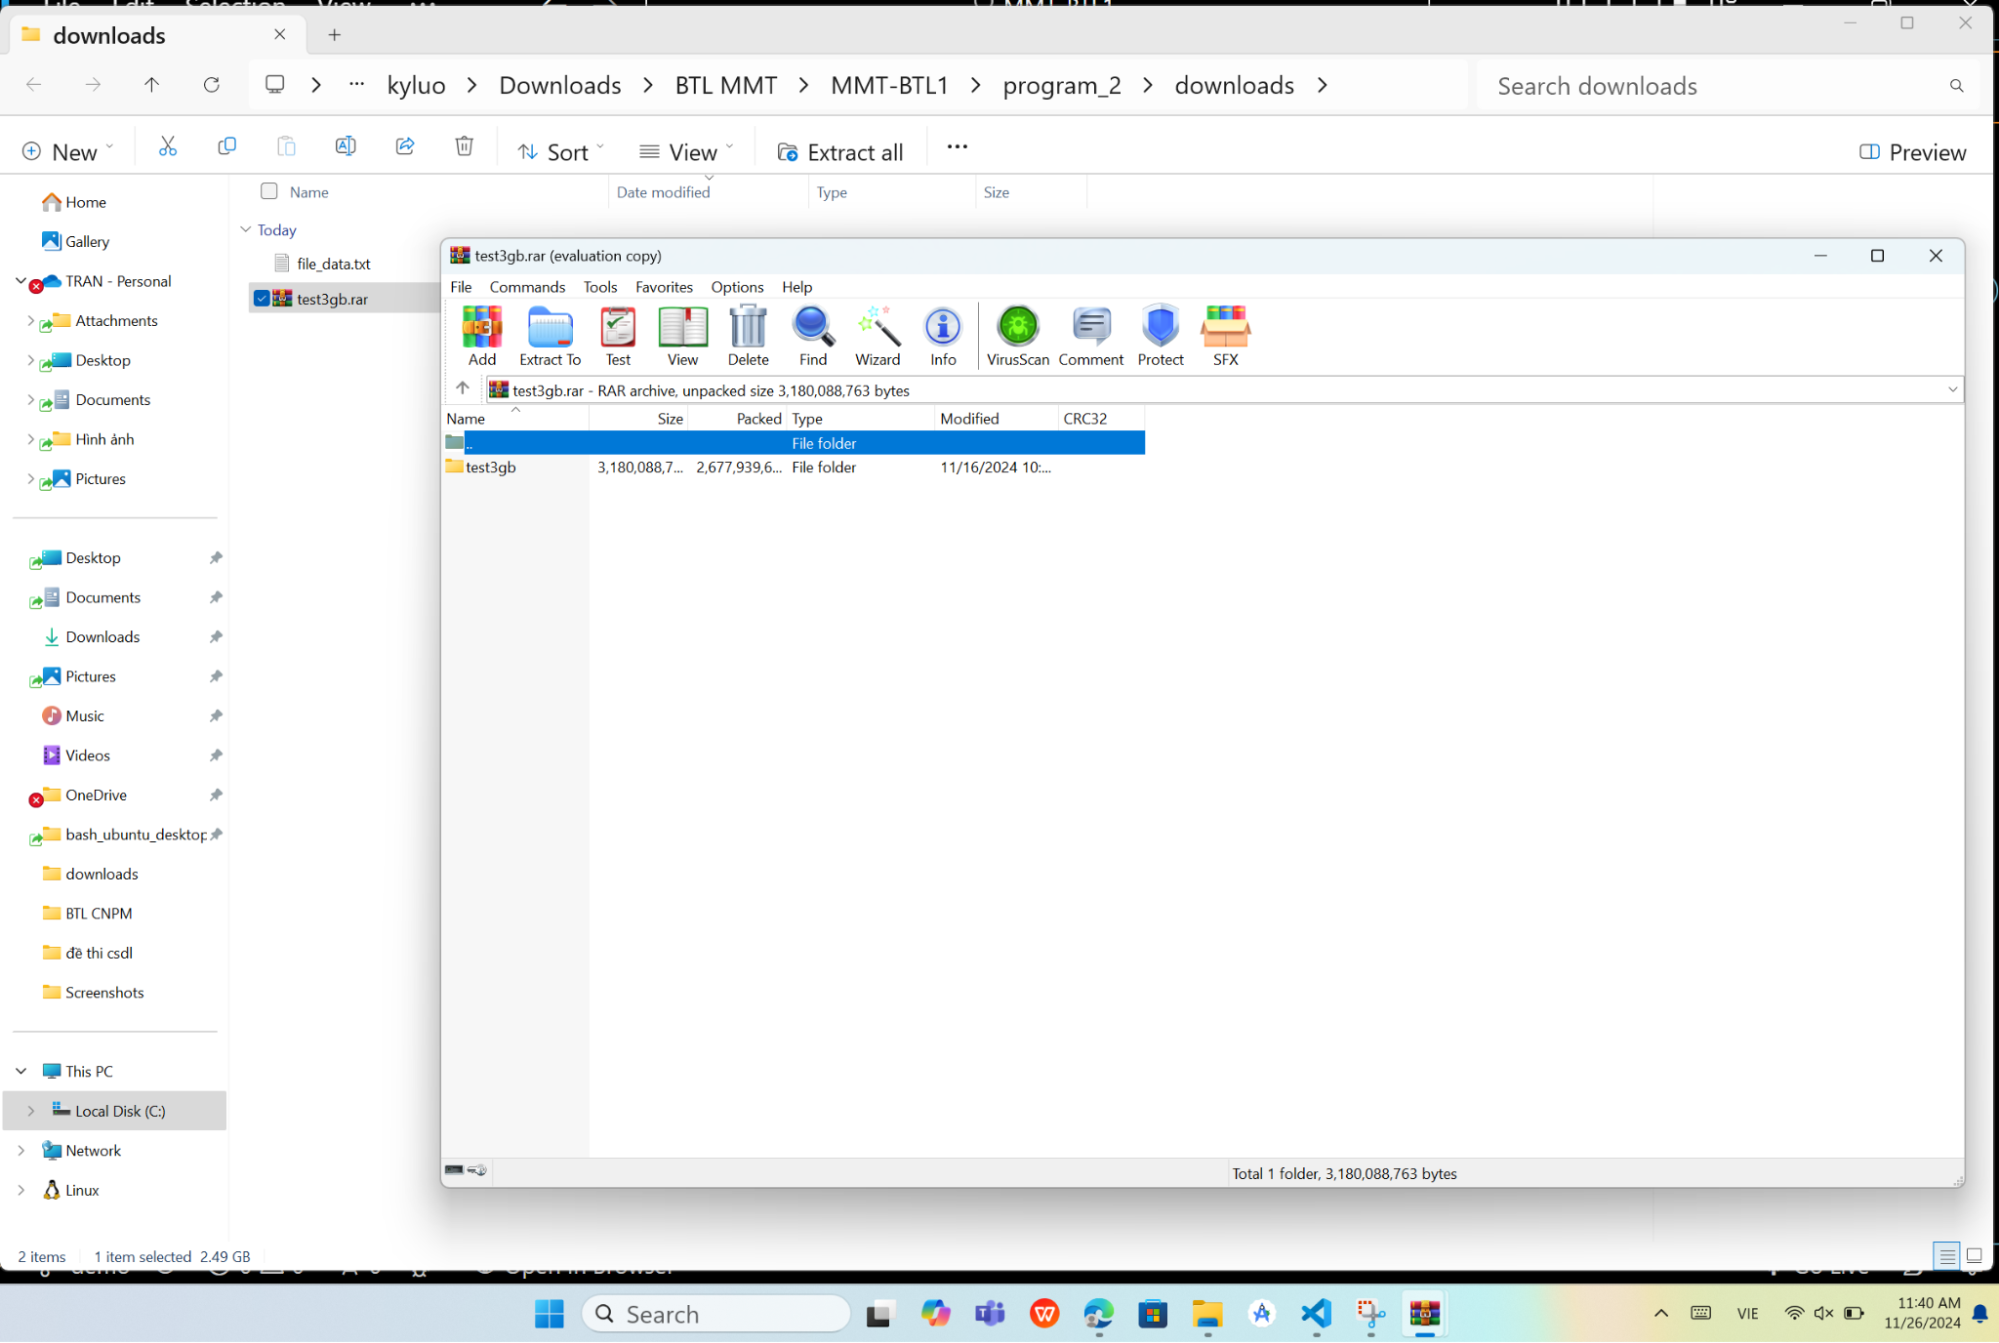
\includegraphics[width=1\textwidth]{images/15.png}
    \captionsetup{labelformat=empty}
    % \caption{MVC}
\end{figure}
\noindent \textbf{CLIENT 3}\\
Trước khi kết nối vào hệ thống, vẫn chưa có file torrent hay file dữ liệu nào trong thư mục \texttt{program\_3}.
\begin{figure}[H]
    \centering
    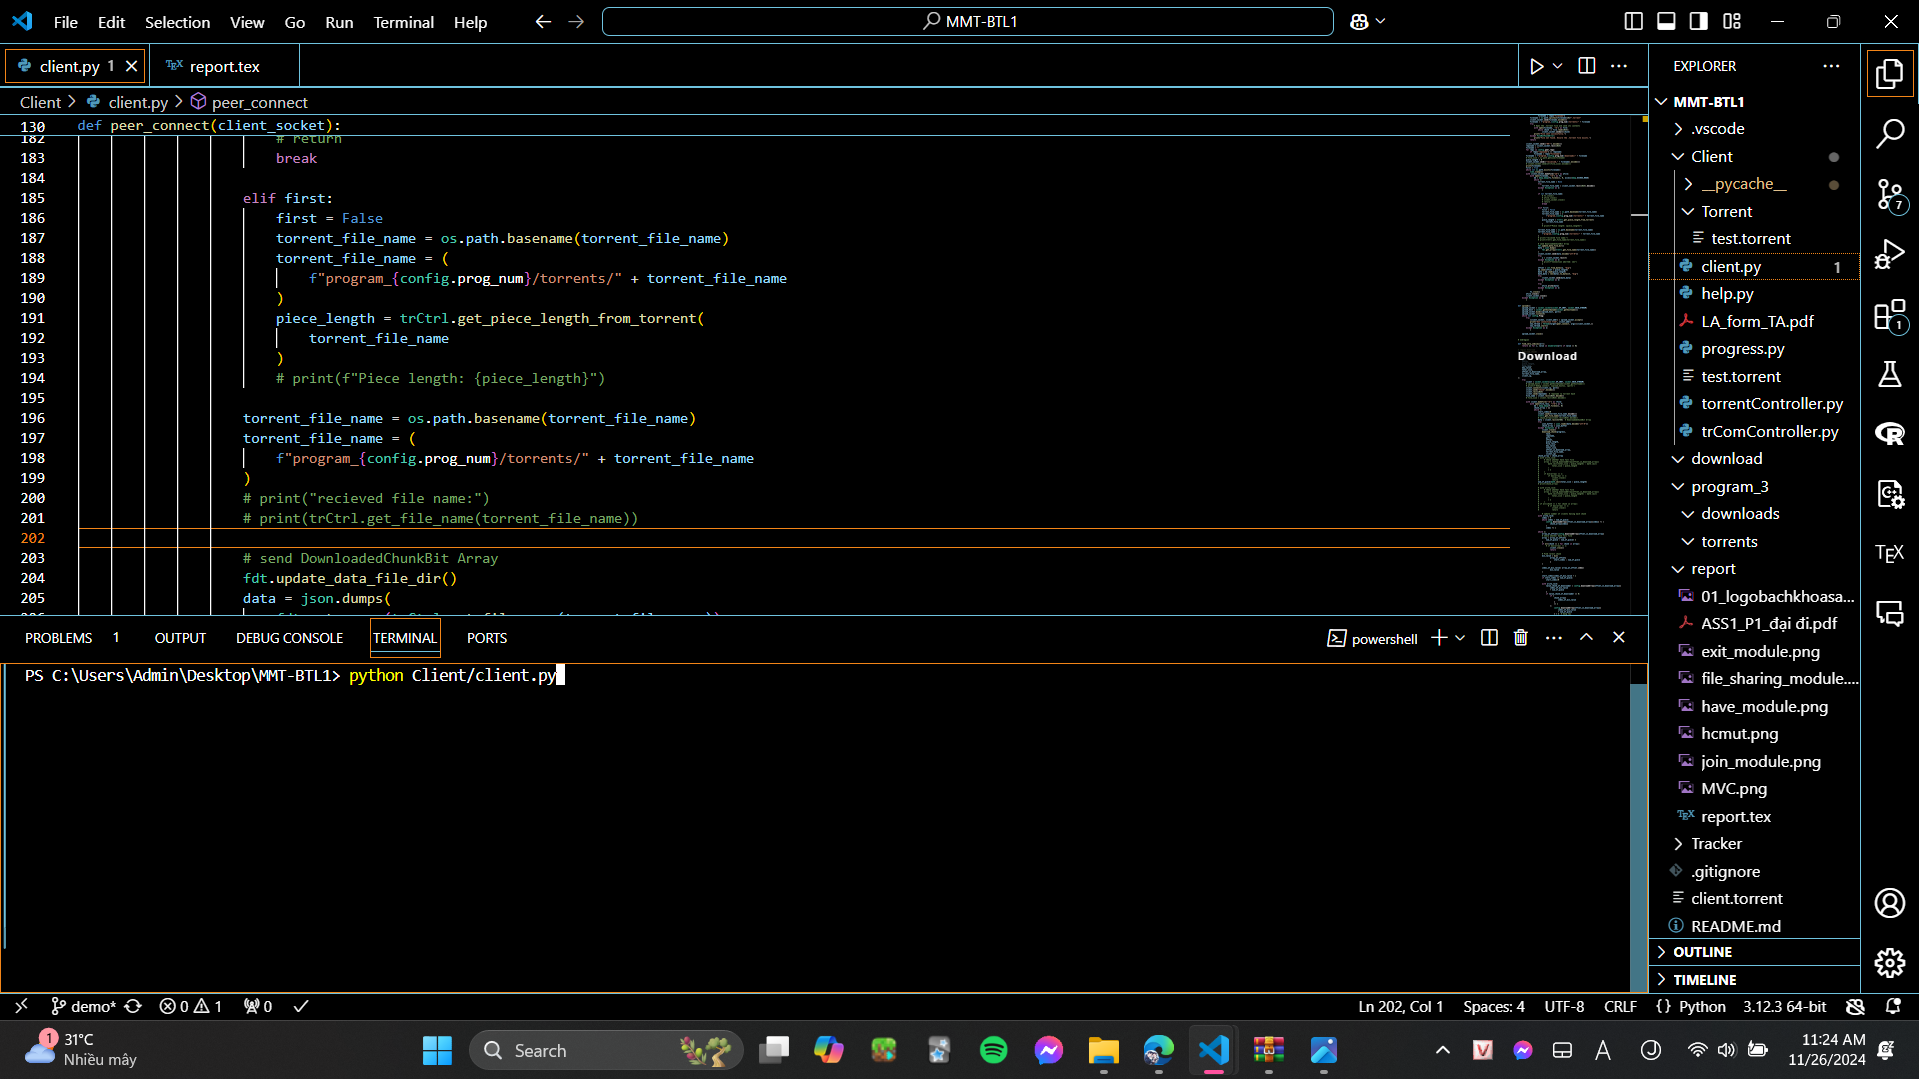
\includegraphics[width=1\textwidth]{images/25.png}
    \captionsetup{labelformat=empty}
    % \caption{MVC}
\end{figure}
Thực hiện chạy chương trình Client.py để chạy một client mới, đồng thời ping cho tracker.
\begin{figure}[H]
    \centering
    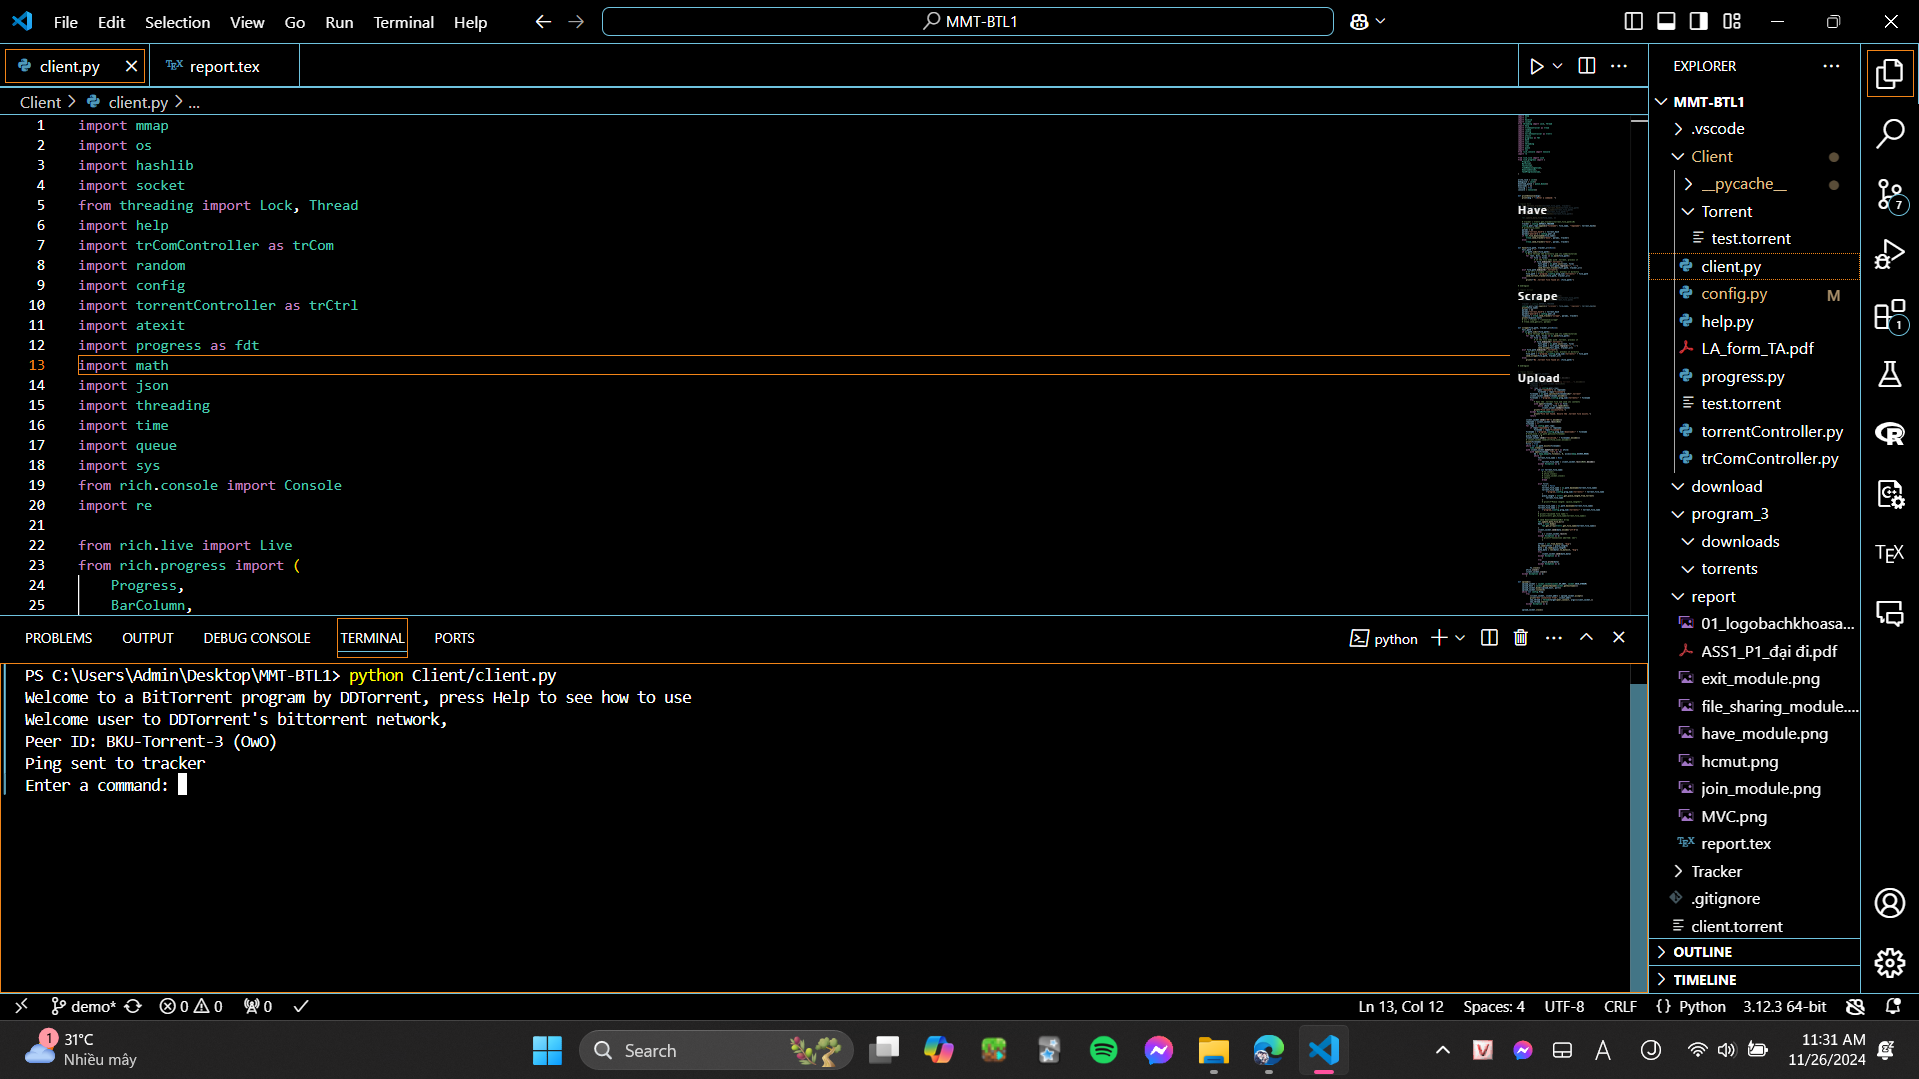
\includegraphics[width=1\textwidth]{images/26.png}
    \captionsetup{labelformat=empty}
    % \caption{MVC}
\end{figure}
Sử dụng lệnh usemagnet + magnet text để download file torrent test3gb.torrent
\begin{figure}[H]
    \centering
    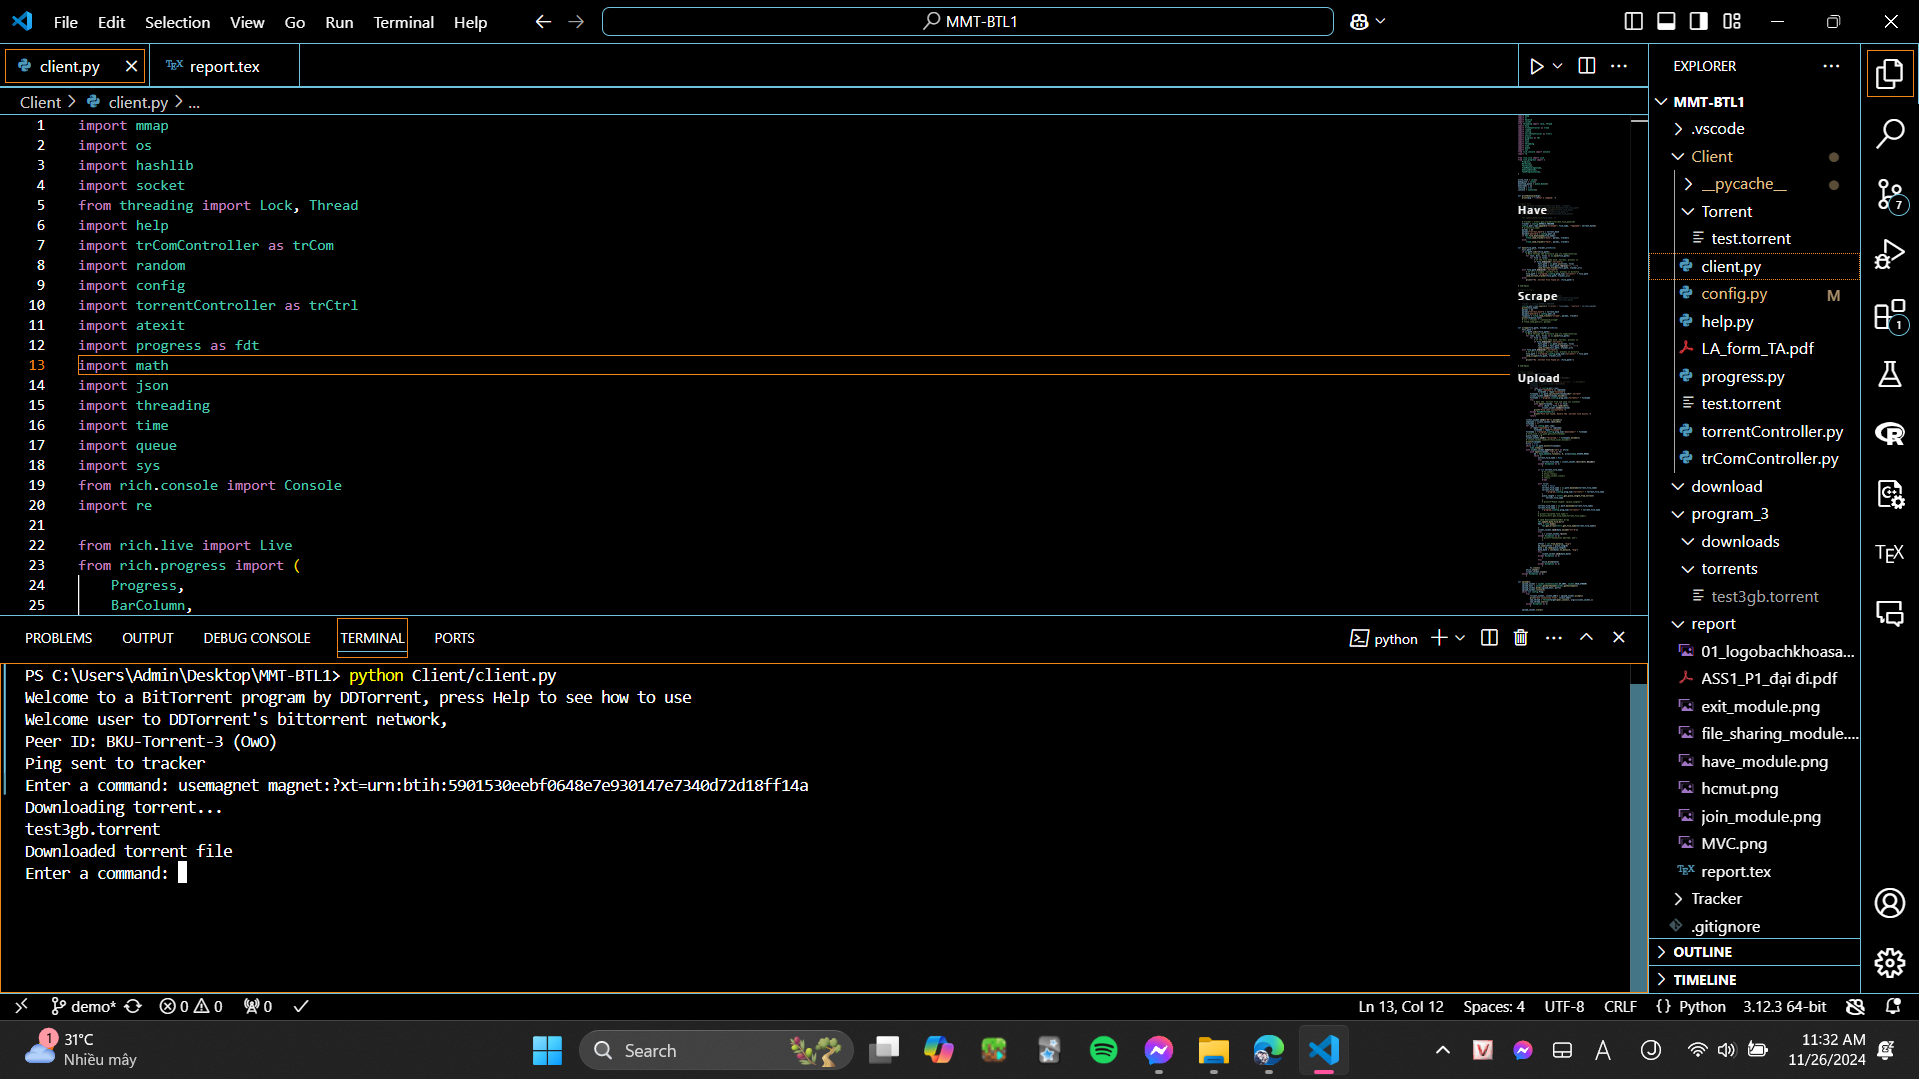
\includegraphics[width=1\textwidth]{images/27.png}
    \captionsetup{labelformat=empty}
    % \caption{MVC}
\end{figure}
Tiếp tục sử dụng usemagnet để download file test1gb.torrent
\begin{figure}[H]
    \centering
    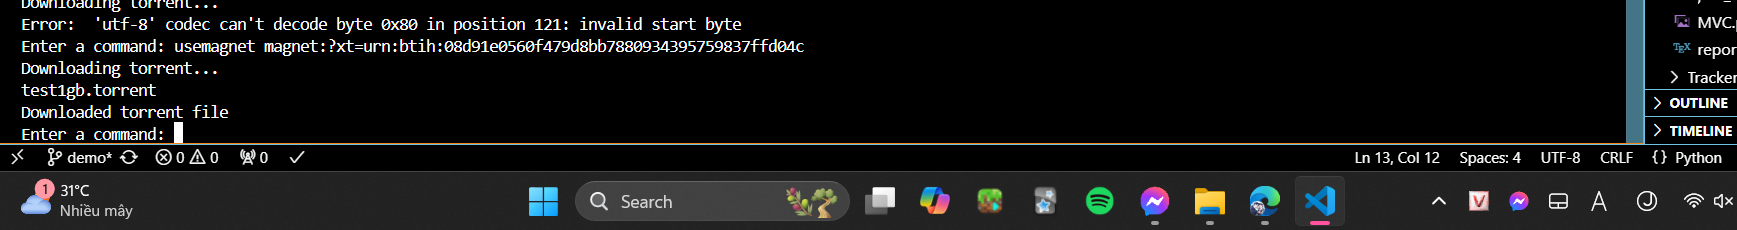
\includegraphics[width=1\textwidth]{images/28.png}
    \captionsetup{labelformat=empty}
    % \caption{MVC}
\end{figure}
Sau khi download 2 file torrent, ta dùng lệnh down + tên torrent file để download đồng thời 2 file test3gb.rar và test1gb.rar
\begin{figure}[H]
    \centering
    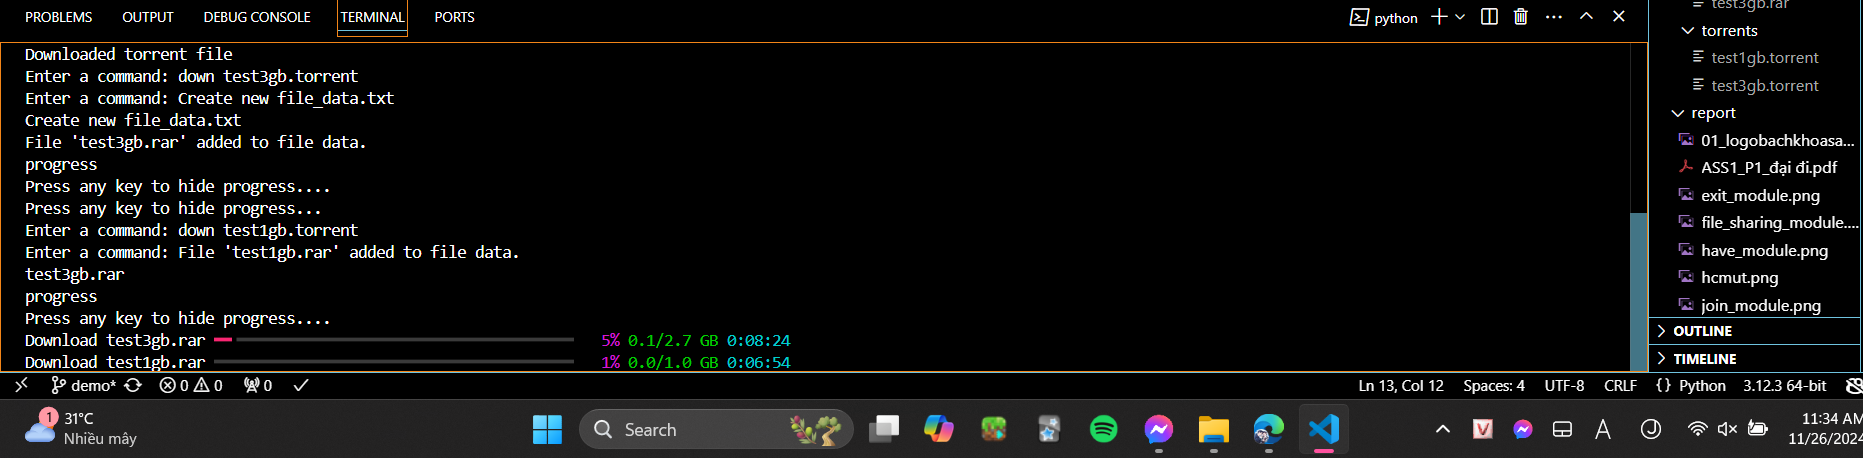
\includegraphics[width=1\textwidth]{images/29.png}
    \captionsetup{labelformat=empty}
    % \caption{MVC}
\end{figure}
Sau đó, sử dụng lệnh progress để xem quá trình download và thời gian còn lại phải chờ.
\begin{figure}[H]
    \centering
    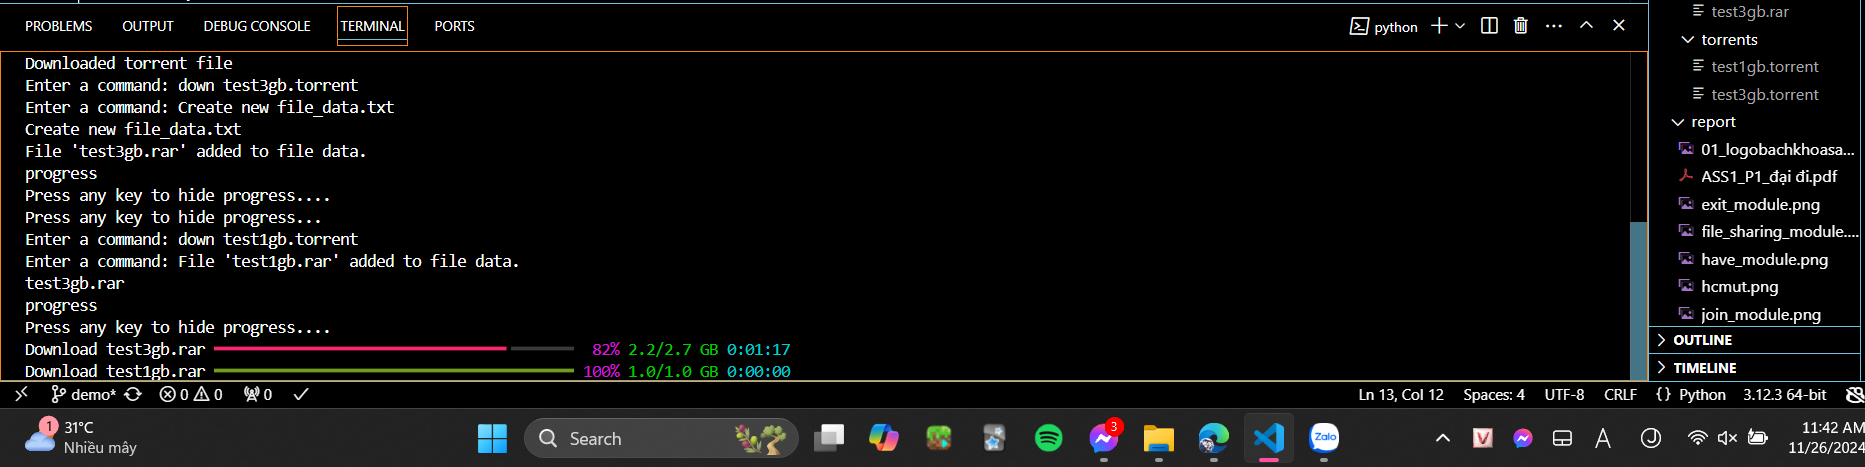
\includegraphics[width=1\textwidth]{images/30.png}
    \captionsetup{labelformat=empty}
    % \caption{MVC}
\end{figure}
Trong lúc đang download thì có peer khác kết nối để nhận file test3gb.rar(Client 4)
\begin{figure}[H]
    \centering
    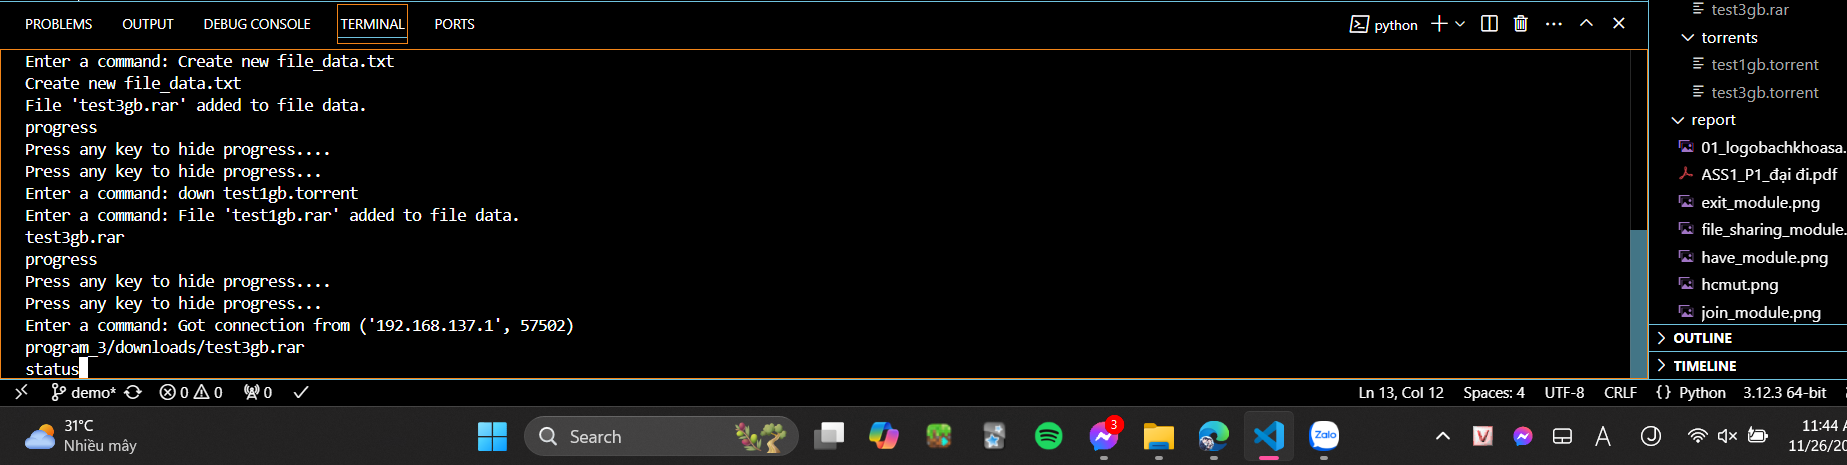
\includegraphics[width=1\textwidth]{images/31.png}
    \captionsetup{labelformat=empty}
    % \caption{MVC}
\end{figure}
Các kết nối client 1 nhận được từ các client 2 và 3 cho đến thời điểm 11:34
\begin{figure}[H]
    \centering
    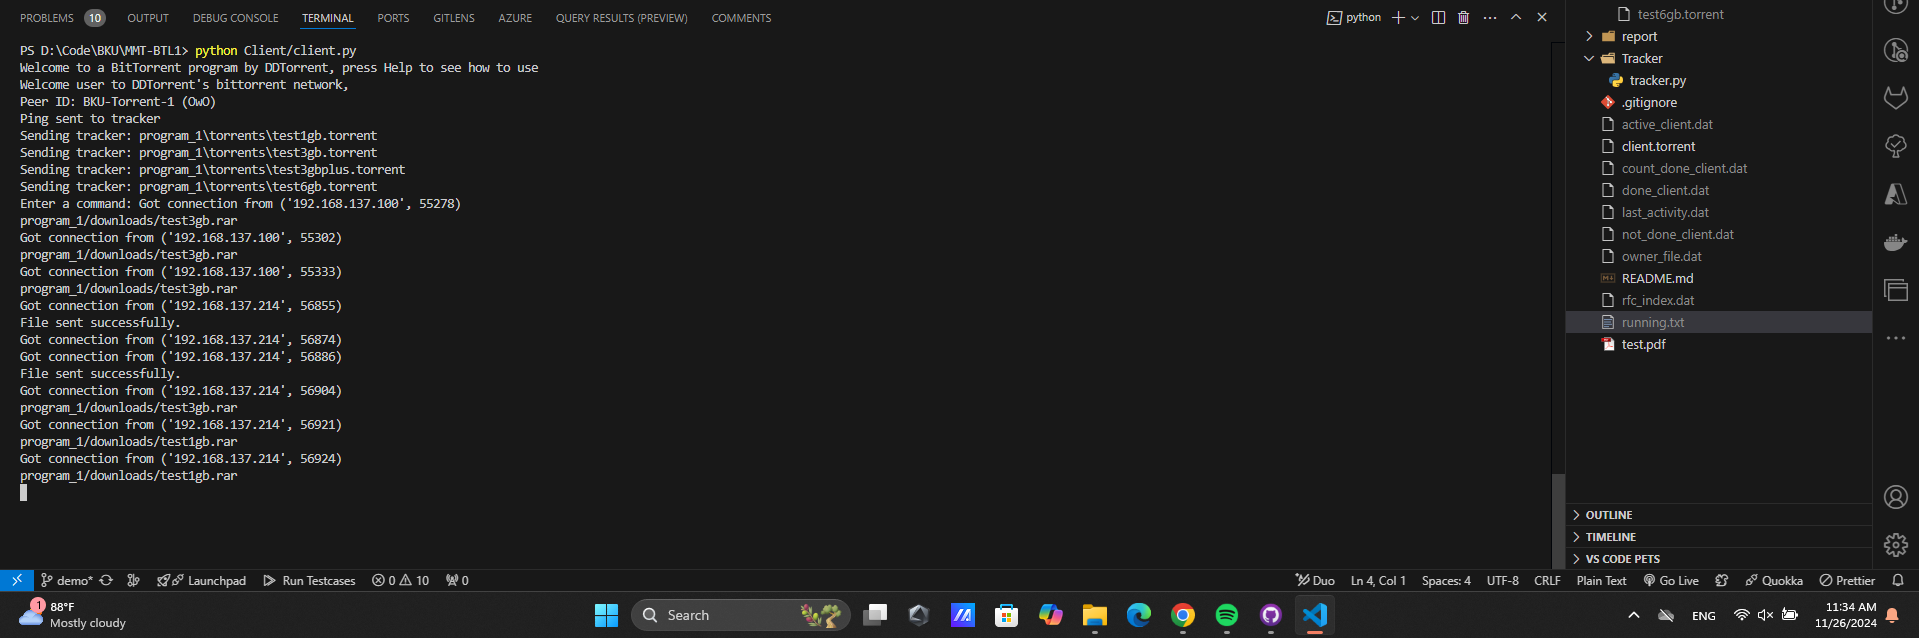
\includegraphics[width=1\textwidth]{images/16.png}
    \captionsetup{labelformat=empty}
    % \caption{MVC}
\end{figure}
Client 4 vào hệ thống torrent bắt đầu download file test3gb.rar tại thời điểm (11:44)
\begin{figure}[H]
    \centering
    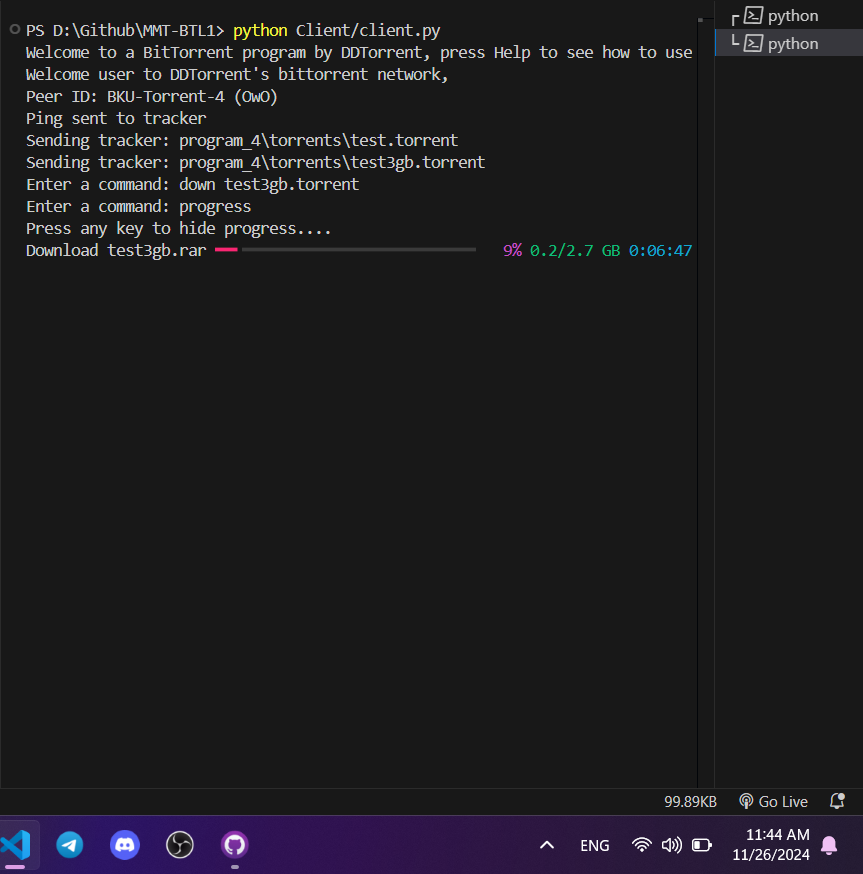
\includegraphics[width=1\textwidth]{images/17.png}
    \captionsetup{labelformat=empty}
    % \caption{MVC}
\end{figure}

\noindent \textbf{SERVER}
Server nhận lệnh done từ client 3 (Client 3 thông báo đã tải xong file có mã \texttt{torrent\_hash}.)	
\begin{figure}[H]
    \centering
    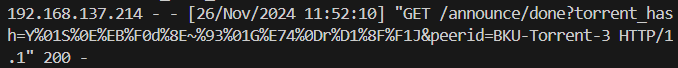
\includegraphics[width=1\textwidth]{images/33.png}
    \captionsetup{labelformat=empty}
    % \caption{MVC}
\end{figure}
Nhận lệnh have từ client 4 (Client 4 thông báo đang có file torrent)
\begin{figure}[H]
    \centering
    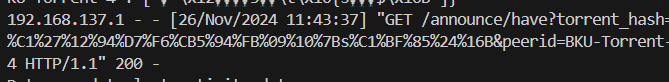
\includegraphics[width=1\textwidth]{images/18.png}
    \captionsetup{labelformat=empty}
    % \caption{MVC}
\end{figure}
Nhận được kết nối từ client 4
\begin{figure}[H]
    \centering
    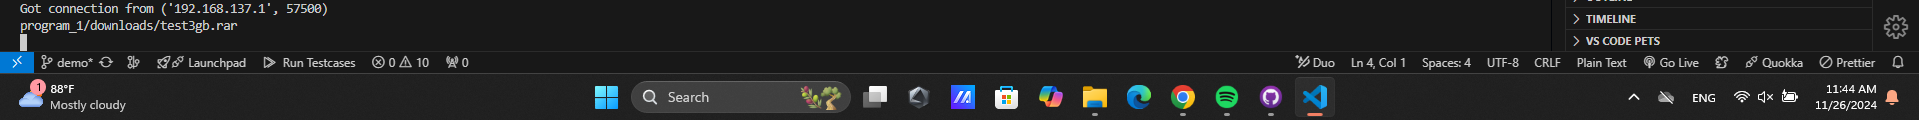
\includegraphics[width=1\textwidth]{images/19.png}
    \captionsetup{labelformat=empty}
    % \caption{MVC}
\end{figure}
Client 2 cũng nhận được kết nối từ client 3 (tải 2 file) và client 4 và upload file cho các Client nếu có file.
\begin{figure}[H]
    \centering
    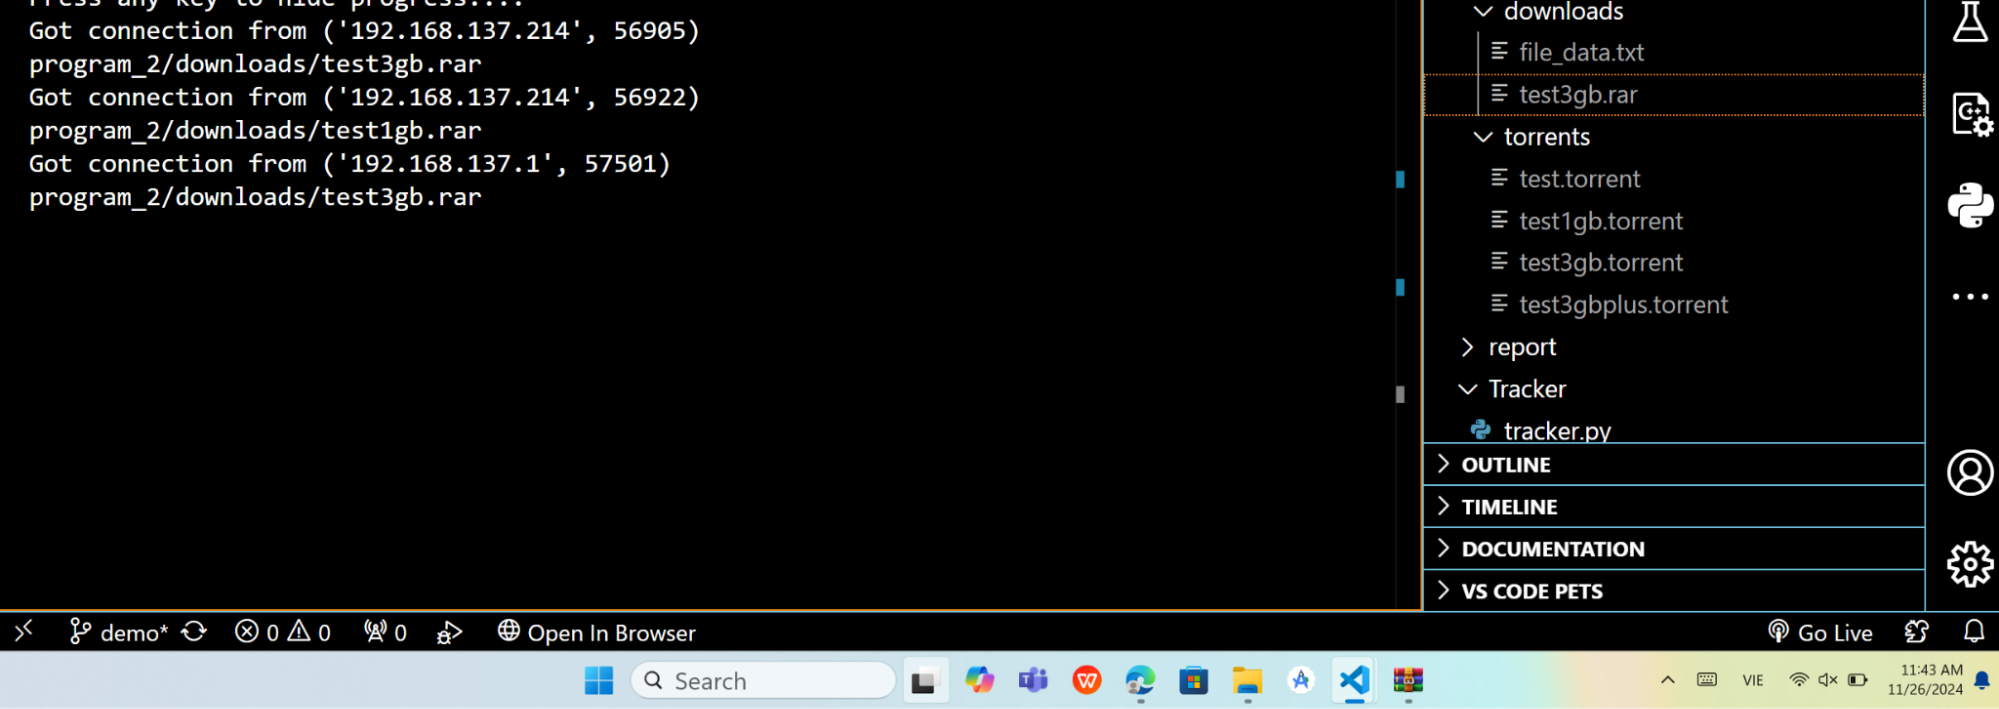
\includegraphics[width=1\textwidth]{images/20.png}
    \captionsetup{labelformat=empty}
    % \caption{MVC}
\end{figure}
Client 4 hoàn thành tải xong
\begin{figure}[H]
    \centering
    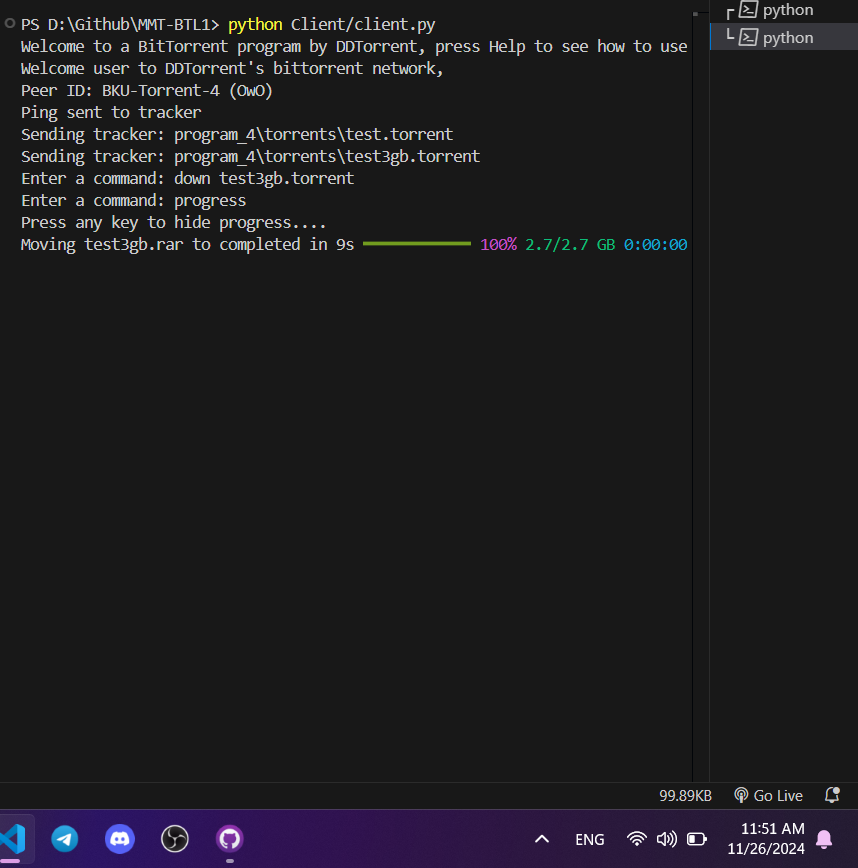
\includegraphics[width=1\textwidth]{images/21.png}
    \captionsetup{labelformat=empty}
    % \caption{MVC}
\end{figure}
Cuối cùng ta sẽ trả về trạng thái của các file trong client 2
\begin{figure}[H]
    \centering
    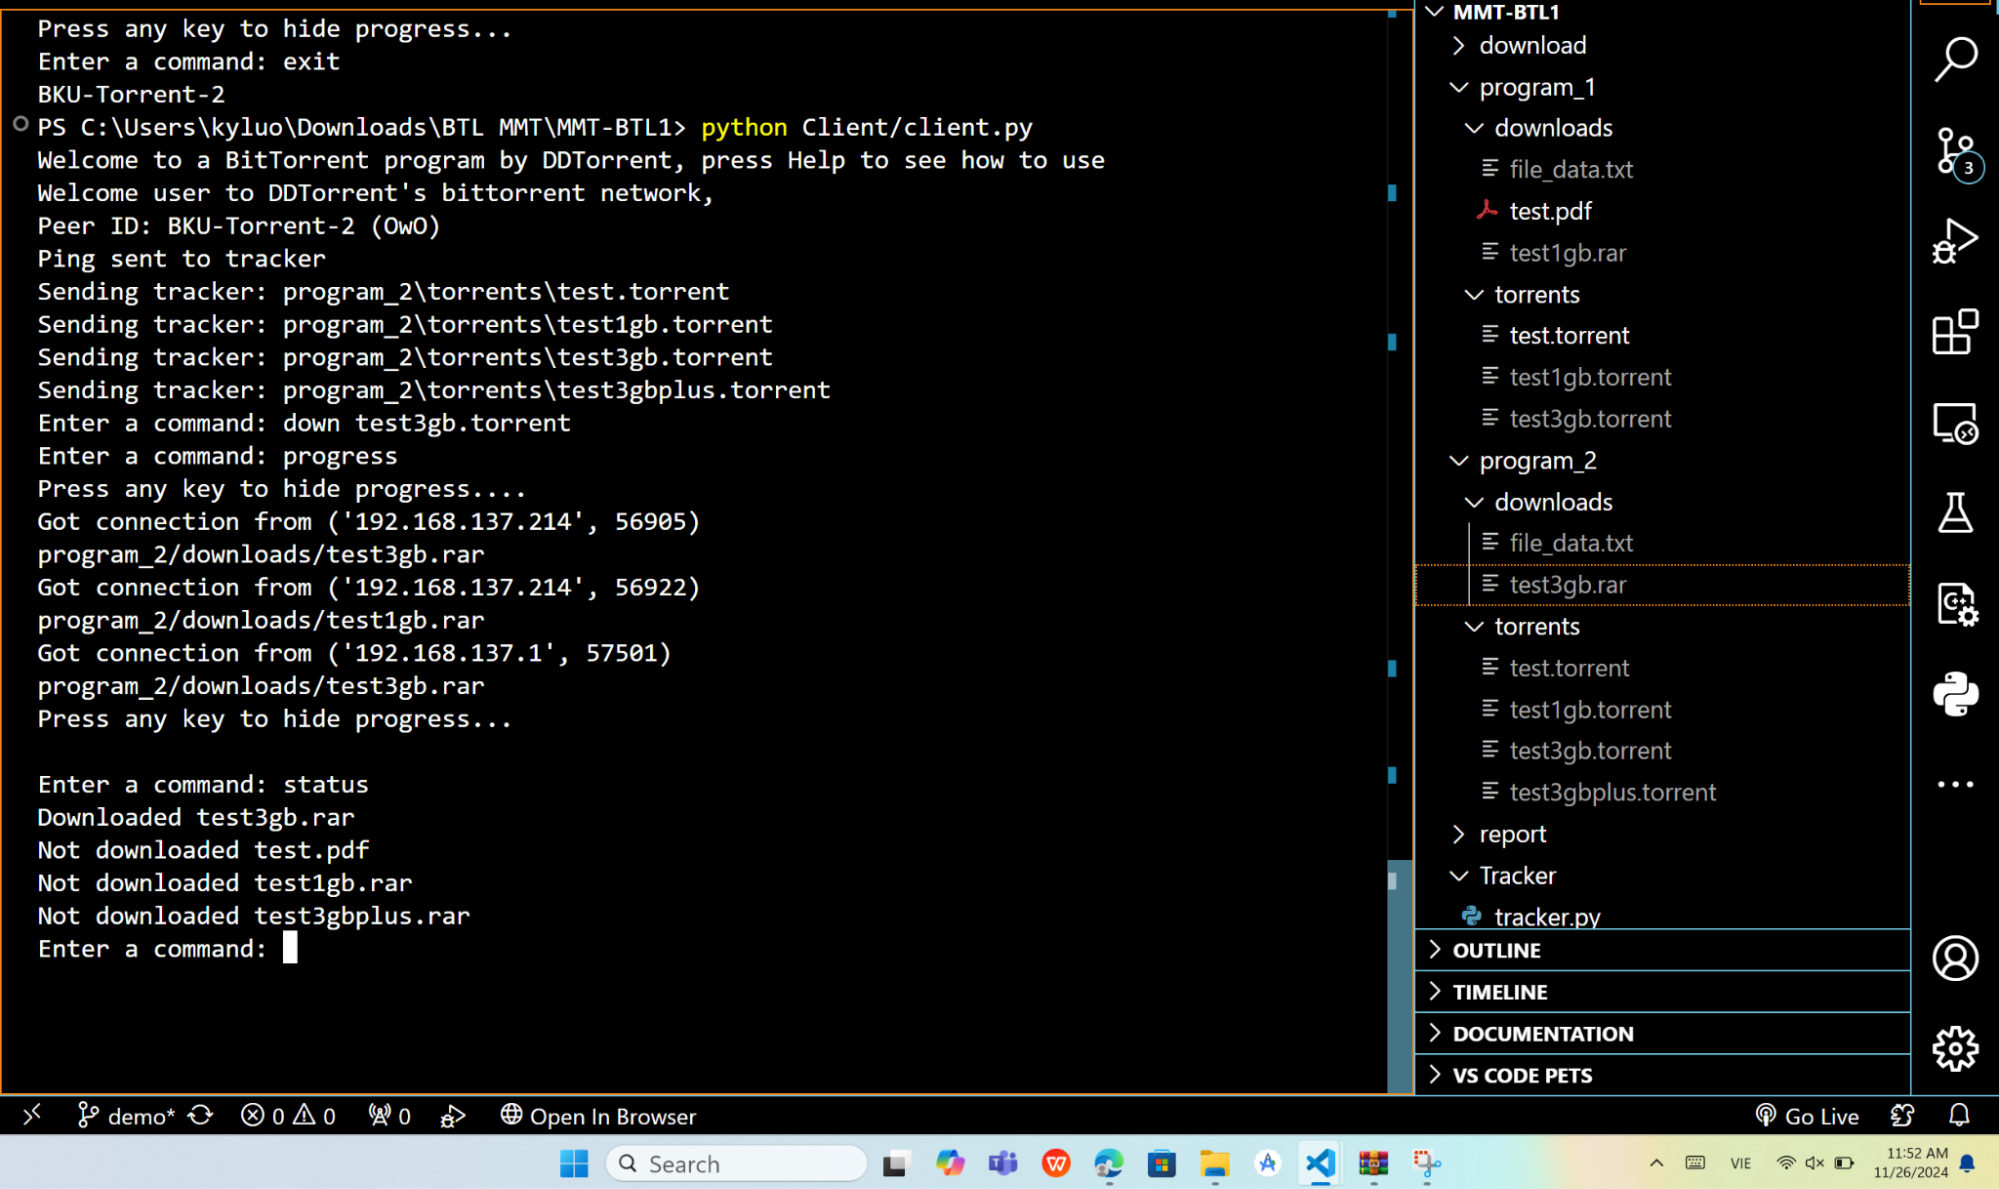
\includegraphics[width=1\textwidth]{images/22.png}
    \captionsetup{labelformat=empty}
    % \caption{MVC}
\end{figure}
Cuối cùng ta sẽ trả về trạng thái của các file trong client 3
\begin{figure}[H]
    \centering
    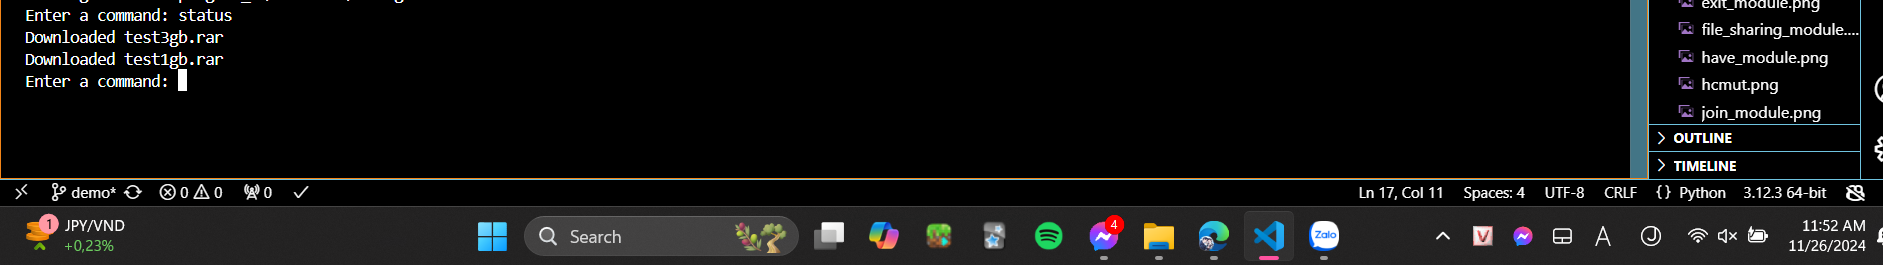
\includegraphics[width=1\textwidth]{images/32.png}
    \captionsetup{labelformat=empty}
    % \caption{MVC}
\end{figure}
Cuối cùng ta sẽ trả về trạng thái của các file trong client 4
\begin{figure}[H]
    \centering
    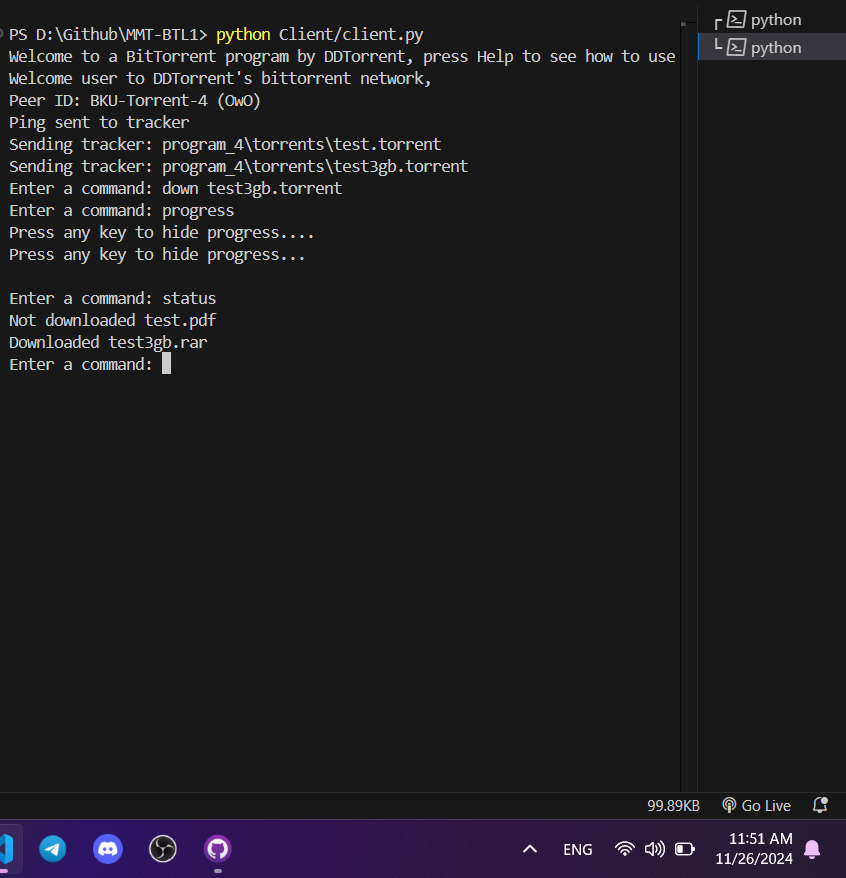
\includegraphics[width=1\textwidth]{images/23.png}
    \captionsetup{labelformat=empty}
    % \caption{MVC}
\end{figure}
\indent CLIENT 4:\\
File mở thành công
\begin{figure}[H]
    \centering
    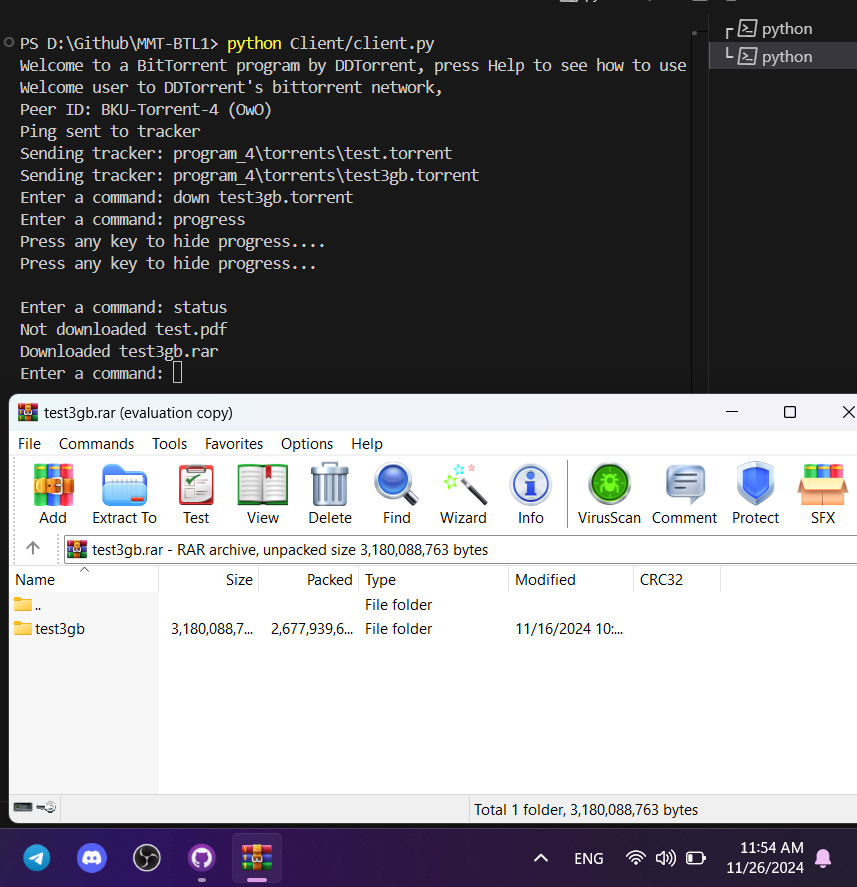
\includegraphics[width=0.8\textwidth]{images/24.png}
    \captionsetup{labelformat=empty}
    % \caption{MVC}
\end{figure}
\indent CLIENT 3:
\begin{figure}[H]
    \centering
    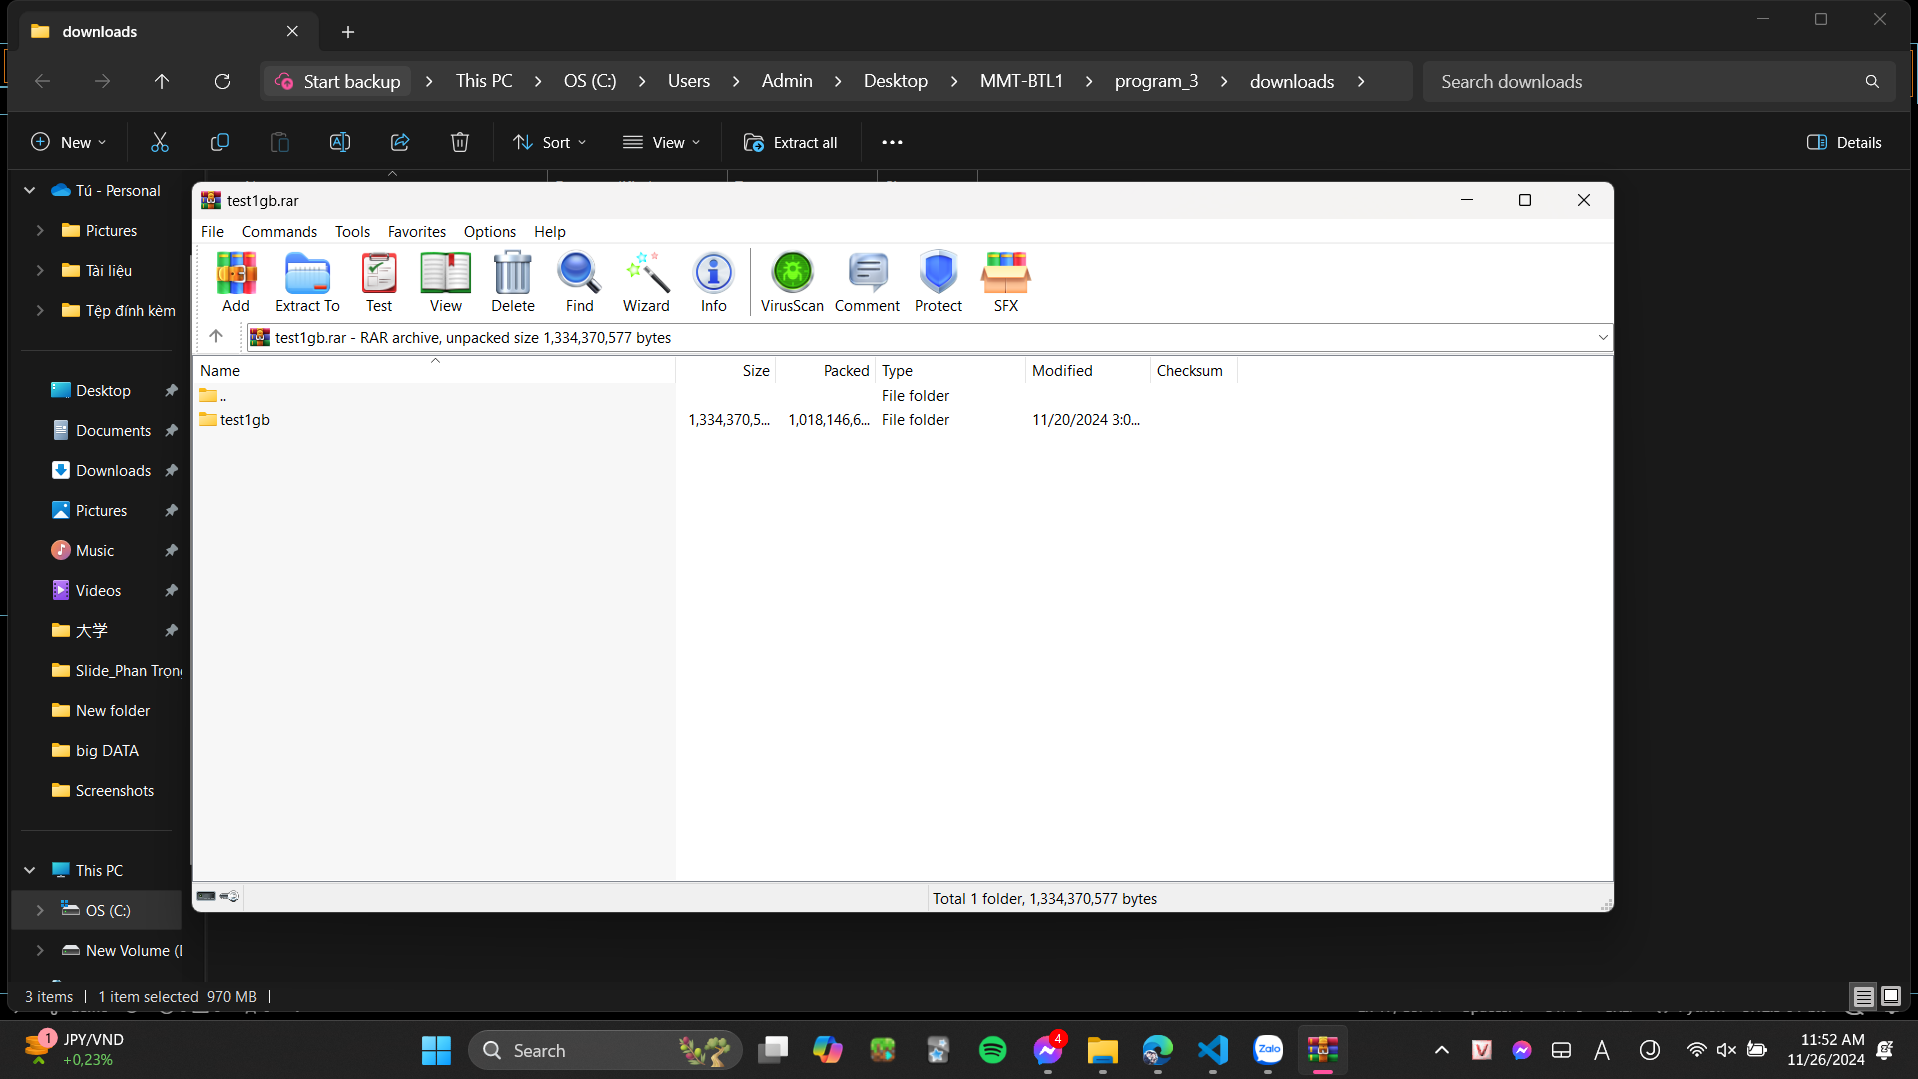
\includegraphics[width=0.8\textwidth]{images/34.png}
    \captionsetup{labelformat=empty}
    % \caption{MVC}
\end{figure}
\begin{figure}[H]
    \centering
    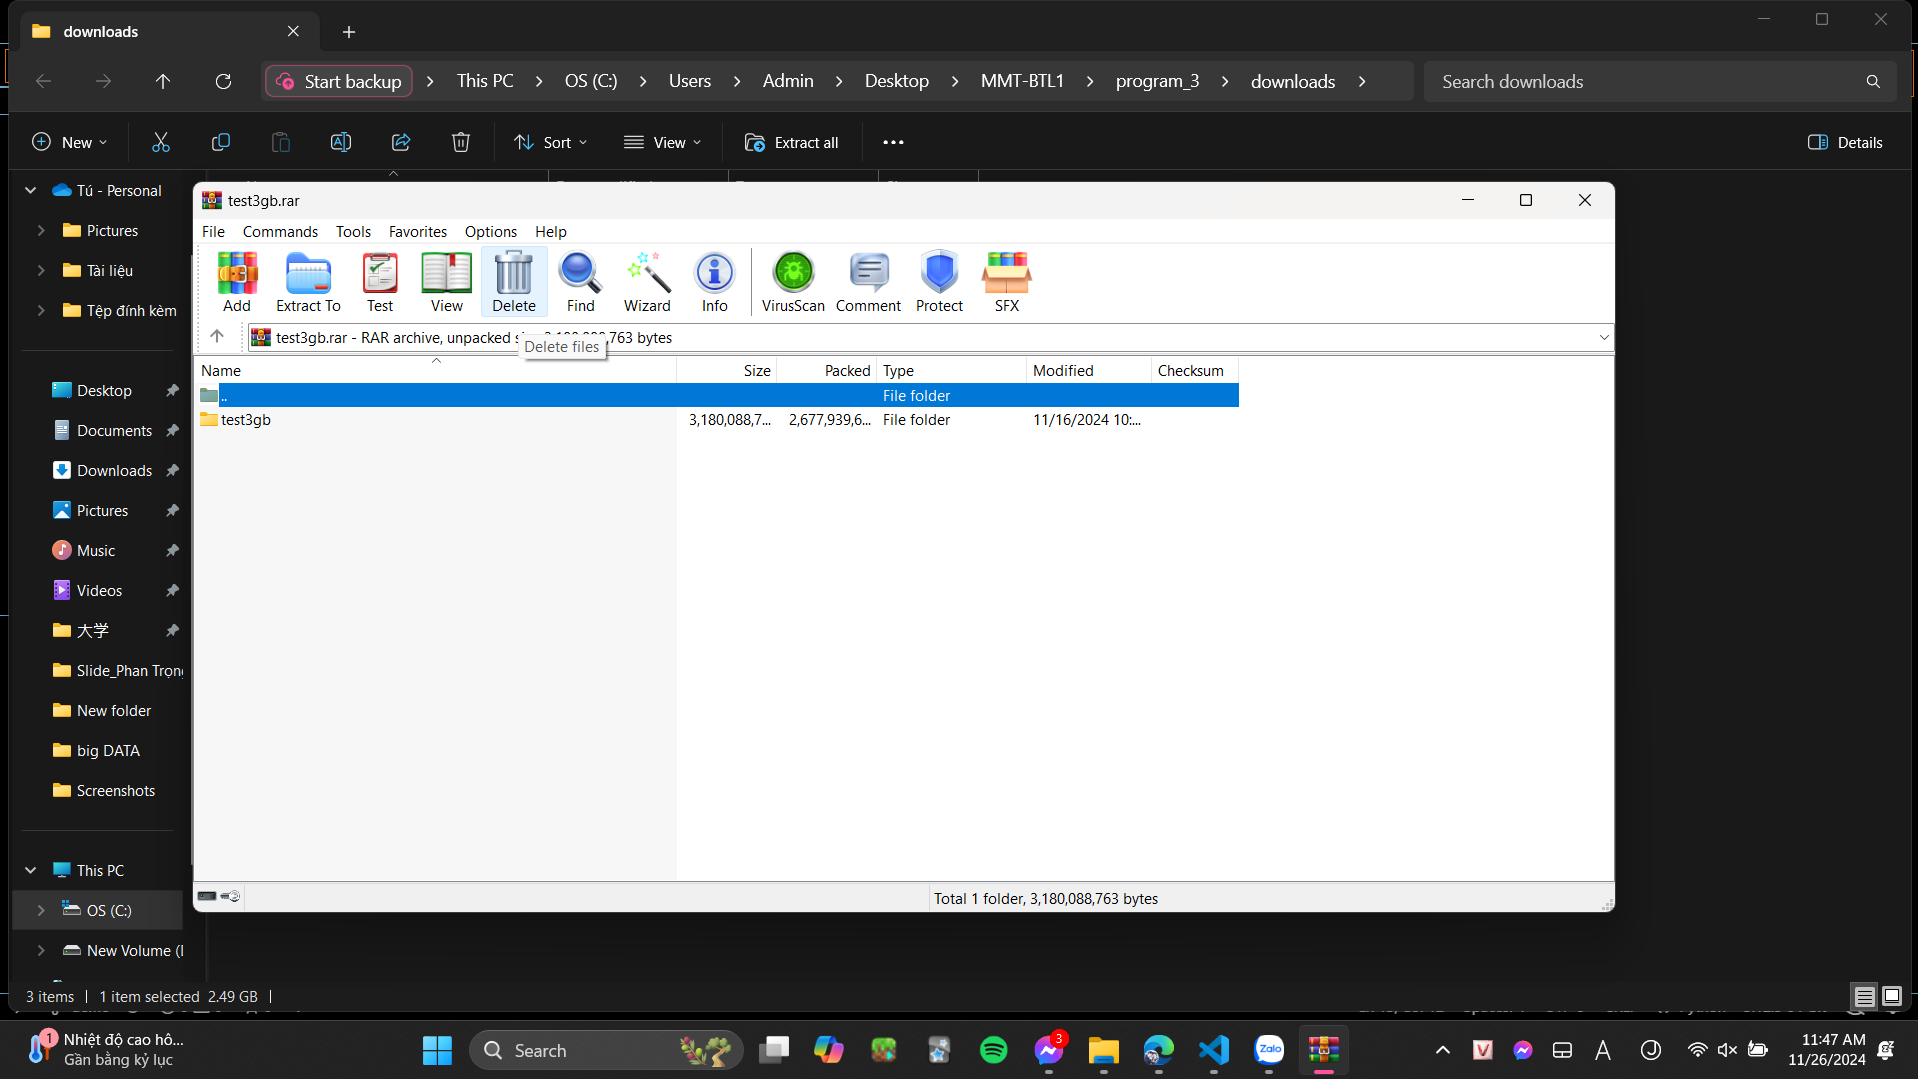
\includegraphics[width=0.8\textwidth]{images/35.png}
    \captionsetup{labelformat=empty}
    % \caption{MVC}
\end{figure}
\subsection{CÁC LỆNH KHÁC}
\noindent \textbf{SCRAPE:}\\
Tại bất kỳ thời điểm, các client có thể sử dụng lệnh scrape để xem có bao nhiêu seeder và leecher cho file torrent test3gbplus để có thể quyết định nên tải file torrent này không hoặc kiếm file khác có nhiều seeder hơn
\begin{figure}[H]
    \centering
    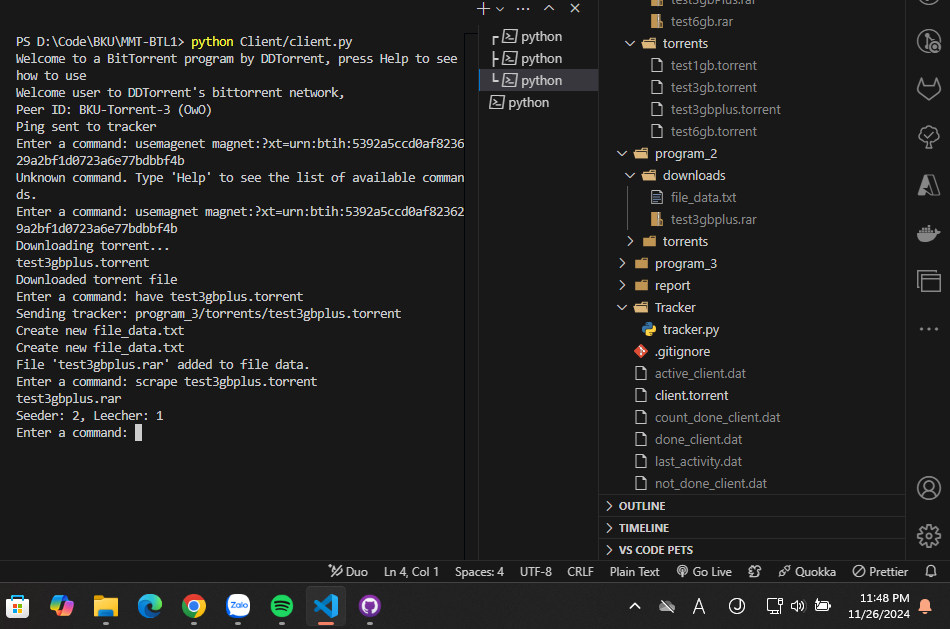
\includegraphics[width=1\textwidth]{images/39.png}
    \captionsetup{labelformat=empty}
    % \caption{MVC}
\end{figure}
\noindent \textbf{SERVER:}\\
\indent - Join:
\begin{figure}[H]
    \centering
    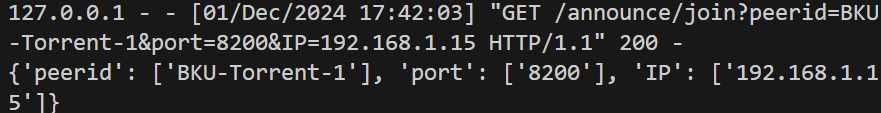
\includegraphics[width=1\textwidth]{images/36.png}
    \captionsetup{labelformat=empty}
    % \caption{MVC}
\end{figure}
- Đưa client vào danh sách hoạt động
\begin{figure}[H]
    \centering
    
\includegraphics[width=1\textwidth]{images/37.png}
    \captionsetup{labelformat=empty}
    % \caption{MVC}
\end{figure}
- Exit
\begin{figure}[H]
    \centering
    
\includegraphics[width=1\textwidth]{images/38.png}
    \captionsetup{labelformat=empty}
    % \caption{MVC}
\end{figure}
Thông báo thoát khỏi hệ thống bittorrent cho tracker để tracker xóa client ra khỏi các danh sách liên quan	


\end{document}
